%!TEX root = ../documentation.tex

\documentclass[%
	pdftex,
	oneside,			% Einseitiger Druck.
	11pt,				% Schriftgroesse
	parskip=half,		% Halbe Zeile Abstand zwischen Absätzen.
	headsepline,		% Linie nach Kopfzeile.
	footsepline,		% Linie vor Fusszeile.
	abstracton,			% Abstract Überschriften
	listof=totoc,
	toc=bibliography,
	headings=optiontohead,
	plainfootsepline
]{scrreprt}

%% Schrift -> Muss hier bleiben sonst gibts Probleme mit dem Deckblatt
\usepackage{xstring}
\usepackage[utf8]{inputenc}
\usepackage[T1]{fontenc}
\usepackage{lmodern}
\renewcommand{\familydefault}{\sfdefault} % serifen lose Schriftart

% Sprache
\usepackage[ngerman]{babel}

%% Mathepakete & Schrift
\usepackage{amsmath}
\usepackage{amsthm}
\usepackage{amsbsy}
\usepackage{amssymb}
\usepackage{sansmath}
\sansmath

%% Für Tables/Images/Figures
\usepackage{here}



%% ---------------------- Allgemeine Einstellungen ----------------------

\newcommand{\kurs}{TINF14-AIBC}

\newcommand{\titel}{Entwicklung einer Foto-App für Android} % Titel noch im Beta-Status
%\newcommand{\titelA}{--} % Für längere Titel
%\newcommand{\titelB}{--}


\newcommand{\datumAbgabe}{November 2015}

\newcommand{\abgabeort}{Mannheim}
\newcommand{\studiengang}{Studiengang Angewandte Informatik}
\newcommand{\dhbw}{Mannheim}

\newcommand{\zeitraum}{4 Wochen}
\newcommand{\arbeit}{Studienarbeit}
\newcommand{\autor}{Tobias Dorra und Philipp Pütz}

\newcommand{\sprache}{de}

\newcommand{\spaltenabstand}{10pt}
\newcommand{\zeilenabstand}{1.5}

\newcommand{\artikelstudiengang}{im}
\newcommand{\anderdh}{an der Dualen Hochschule Baden-Württemberg}
\newcommand{\von}{von}

\newcommand{\sperrvermerk}{Sperrvermerk}
\newcommand{\erklaerung}{Erklärung}
\newcommand{\abkverz}{Abkürzungsverzeichnis}
\newcommand{\glossar}{Glossar}


%%%%%%%%%%%%%%%%%%%%%%%%%%%%%%%%%%%%%%%%%%%%%%%%%%%%%%%%%%%%%%%%%%%%%%%%%%%%%%%%


%%%%%%% Package Includes %%%%%%%

\usepackage[a4paper, left=25mm,right=25mm, top=38mm, bottom=43mm]{geometry}
\usepackage[activate]{microtype} %Zeilenumbruch und mehr
\usepackage[onehalfspacing]{setspace}
\usepackage{makeidx}
\usepackage[autostyle=true,german=quotes]{csquotes}
\usepackage{longtable}
\usepackage{graphicx}
\usepackage{calc}		%zum Rechnen (Bildtabelle in Deckblatt)
\usepackage{wrapfig}
\usepackage[perpage, hang, multiple, stable]{footmisc} % Bibverzeichnis
\usepackage[printonlyused,footnote]{acronym}
\usepackage{textcomp}
\usepackage{tabularx}
\usepackage{ltablex}
\usepackage{booktabs}
\usepackage{longtable}

 % Für Codebeispiele
\usepackage{listings}

\usepackage{epstopdf} % Eps Grafikeinbidnung
\usepackage{nameref}

%% Paket um Textteile drehen zu können
\usepackage{rotating}

%% Paket um Seite im Querformat anzuzeigen
\usepackage{lscape}

%% Farben (Angabe in HTML-Notation mit großen Buchstaben)
\usepackage{xcolor} 	%xcolor für HTML-Notation
\definecolor{LinkColor}{HTML}{000000}
\definecolor{ListingBackground}{HTML}{FCF7DE}


%% Programmiersprachen Highlighting (Listings)
\newcommand{\listingsettings}{%
	\lstset{%
		language=Java,			% Standardsprache des Quellcodes
		%numbers=left,			% Zeilennummern links
		stepnumber=1,			% Jede Zeile nummerieren.
		numbersep=5pt,			% 5pt Abstand zum Quellcode
		numberstyle=\tiny,		% Zeichengrösse 'tiny' für die Nummern.
		breaklines=true,		% Zeilen umbrechen wenn notwendig.
		breakautoindent=true,	% Nach dem Zeilenumbruch Zeile einrücken.
		postbreak=\space,		% Bei Leerzeichen umbrechen.
		tabsize=2,				% Tabulatorgrösse 2
		basicstyle=\ttfamily\footnotesize, % Nichtproportionale Schrift, klein für den Quellcode
		showspaces=false,		% Leerzeichen nicht anzeigen.
		showstringspaces=false,	% Leerzeichen auch in Strings ('') nicht anzeigen.
		extendedchars=true,		% Alle Zeichen vom Latin1 Zeichensatz anzeigen.
		captionpos=b,			% sets the caption-position to bottom
		backgroundcolor=\color{ListingBackground}, % Hintergrundfarbe des Quellcodes setzen.
		xleftmargin=0pt,		% Rand links
		xrightmargin=0pt,		% Rand rechts
		frame=single,			% Rahmen an
		frameround=ffff,
		rulecolor=\color{darkgray},	% Rahmenfarbe
		fillcolor=\color{ListingBackground}
	}
}



%%%%%% Configuration %%%%%
% Titel, Autor und Datum

\title{\titel}
\author{\autor}
\date{\datum}

% PDF Einstellungen
\usepackage[%
	pdftitle={\titel},
	pdfauthor={\autor},
	pdfsubject={\arbeit},
	pdfcreator={pdflatex, LaTeX with KOMA-Script},
	pdfpagemode=UseOutlines, 		% Beim Oeffnen Inhaltsverzeichnis anzeigen
	pdfdisplaydoctitle=true, 		% Dokumenttitel statt Dateiname anzeigen.
	pdflang={\sprache}, 			% Sprache des Dokuments.
]{hyperref}

% (Farb-)einstellungen für die Links im PDF
\hypersetup{%
	colorlinks=true, 		% Aktivieren von farbigen Links im Dokument
	linkcolor=LinkColor, 	% Farbe festlegen
	citecolor=LinkColor,
	filecolor=LinkColor,
	menucolor=LinkColor,
	urlcolor=LinkColor,
	linktocpage=true, 		% Nicht der Text sondern die Seitenzahlen in Verzeichnissen klickbar
	bookmarksnumbered=true 	% Überschriftsnummerierung im PDF Inhalt anzeigen.
}

% Workaround um Fehler in Hyperref, muss hier stehen bleiben
\usepackage{bookmark} %nur ein latex-Durchlauf für die Aktualisierung von Verzeichnissen nötig

% Schriftart in Captions etwas kleiner
\addtokomafont{caption}{\small}


% Literaturverweise

\usepackage[
	backend=bibtex,		% empfohlen. Falls biber Probleme macht: bibtex
	bibwarn=true,
	bibencoding=ascii,	% wenn .bib in utf8, sonst ascii
	sortlocale=de_DE,
	style=numeric % 
	%isbn=false,
	%sorting=none,	%Zitierstil. Siehe http://ctan.mirrorcatalogs.com/macros/latex/contrib/biblatex/doc/biblatex.pdf
]{biblatex}


%% ---------------------- Literatur ----------------------
\bibliography{bibliographie}

\setlength{\bibitemsep}{10pt}
\setlength{\bibhang}{50pt}

\setcounter{biburllcpenalty}{7000}
\setcounter{biburlucpenalty}{8000}
\setcounter{biburlnumpenalty}{8000}

% Hurenkinder und Schusterjungen verhindern
% http://projekte.dante.de/DanteFAQ/Silbentrennung
\clubpenalty=10000
\widowpenalty=10000
\displaywidowpenalty=10000


\setlength{\tabcolsep}{\spaltenabstand}
\renewcommand{\arraystretch}{\zeilenabstand}

%% Header und Footer
\usepackage[autooneside=false,automark]{scrlayer-scrpage}
   
\clearpairofpagestyles
\cfoot*{\pagemark}
\ihead{\ifstr{\rightbotmark}{\leftmark}{}{\rightbotmark}}
\ohead{\leftmark}

\begin{document}
	
	% Deckblatt
	\begin{spacing}{1}
		%!TEX root = ../documentation.tex

\begin{titlepage}
	\begin{longtable}{p{8.0cm} p{5.4cm}}
		%{\raisebox{\ht\strutbox-\totalheight}{\includegraphics[scale=0.6]{images/unser_logo}}} & % Hier könnte unser Logo stehen
		{\raisebox{\ht\strutbox-\totalheight}{
\includegraphics[scale=0.17]{images/dhbw.png}}} % Logo ist noch falsch positioniert, da das andere fehlt
	\end{longtable}
	\enlargethispage{20mm}
	\begin{center}
		\vspace*{12mm}	{\sffamily\LARGE\textbf{\titel}}\\
		%\vspace*{3mm}	{\sffamily\LARGE\textbf{\titelB}}\\
		\vspace*{12mm}	{\large\textbf{\arbeit}}\\
        \vspace*{12mm}	\artikelstudiengang{} \studiengang\\
        \vspace*{3mm}   \anderdh{} \dhbw\\
		\vspace*{12mm}	\von\\
		\vspace*{3mm}	{\large\textbf{\autor}}\\
		\vspace*{12mm}	\datumAbgabe\\
	\end{center}
	\vfill
	\begin{spacing}{1.2}
	\begin{tabbing}
		mmmmmmmmmmmmmmmmmmmmmmmmmmmmmmmmmmmmmm  \= \kill
		\textbf{Bearbeitungszeitraum}           \>  \zeitraum\\
		\textbf{Kurs}               			\>  \kurs\\ %% Matrikelnummmern einfügen?!
	\end{tabbing}
	\end{spacing}
\end{titlepage}

	\end{spacing}
	\newpage

	%  Abstract evtl. wenn benötigt
	% %!TEX root = ../dokumentation.tex

\pagestyle{empty}
\renewcommand{\abstractname}{Zusammenfassung} % Text für Überschrift
\begin{abstract}
Meine Zusammenfassung
\end{abstract}

	% \newpage
	
	% Inhaltsverzeichnis
	\begin{spacing}{1.1}
		\setcounter{tocdepth}{1}
		
		%für die Anzeige von Unterkapiteln im Inhaltsverzeichnis
		%\setcounter{tocdepth}{2}
		
		\tableofcontents
		\thispagestyle{empty}
		
	\end{spacing}
	\newpage
	
	% römische Ziffern für Verzeichnisse am Anfang
	\pagenumbering{roman}
	\setcounter{page}{1}
	
	% Abkürzungsverzeichnis
	%\cleardoublepage
	%\phantomsection \label{listofacs}
	%\addcontentsline{toc}{chapter}{\abkverz}
	%%!TEX root = ../documentation.tex

\chapter*{\abkverz}
%nur verwendete Akronyme werden letztlich im Dokument angezeigt
\begin{acronym}[YTMMM]
\setlength{\itemsep}{-\parsep}

\acro{TEST}{TEST}

\end{acronym}


	% Abbildungsverzeichnis
	\cleardoublepage
	\listoffigures	
	
	% Schreibe Seitenzahlen etc. fertig
    \cleardoublepage
    
    % Ändere Pagestyle & Numerierung auf Arabisch
	\pagestyle{scrheadings}	
	\pagenumbering{arabic}
	\setcounter{page}{1}
	
	
	%%%% Kapitel import
	%!TEX root = ../documentation.tex

\chapter{Einführung}

Bei gemeinsamen Freizeitaktivitäten mit Freunden entstehen oft viele Fotos. Diese werden dann entweder gar nicht oder erst Wochen später miteinander geteilt.

Unser Ziel ist es, die Benutzererfahrung beim Teilen der Bilder zu verbessern. Das soll mit einer eigenen Foto-App passieren. Anstatt die gesammelten Bilder erst nach der Veranstaltung auszuwählen und dann an die entsprechenden Kontakte zu schicken, sollen die geschossenen Bilder bereits während der Veranstaltung automatisch mit den anderen anwesenden Freunden geteilt werden.

\section{Funktionen}

\subsection{Organisation der Fotos}
Die Fotos werden in sogenannten \enquote{Streams} gruppiert. Jeder Stream repräsentiert dabei ein gemeinsames Erlebnis mit Freunden. Streams können umbenannt oder gelöscht werden. Beim Löschen eines Streams werden alle enthaltenen Bilder ebenfalls gelöscht.

Um einen Stream mit Fotos zu befüllen, kann entweder die Gerätekamera genutzt werden, oder es werden Fotos aus der Android-Galerie importiert. Die Fotos werden mit Name und Vorschaubild im Stream angezeigt. Außerdem existiert eine Detailansicht, in der man das Foto vergrößert betrachten kann. Fotos können umbenannt oder gelöscht werden. Ausgewählte Fotos können wieder zurück in die Android-Galerie exportiert, oder über die Teilen-Funktion anderen Apps zugänglich gemacht werden.

\subsection{Teilen von Fotos}
Zu einem Stream können mehrere Benutzer hinzugefügt werden. Die Fotos in einem Stream werden live zwischen allen Teilnehmern synchronisiert.

Alle Teilnehmer in einem Stream sind gleichberechtigt. Es gibt also keinen \enquote{Streamadministrator} mit besonderen Rechten. Jeder Teilnehmer eines Streams kann Bilder hinzufügen, Bilder löschen und die Teilnehmerliste verwalten. Insbesondere ist jeder Teilnehmer auch dazu berechtigt, weitere Teilnehmer hinzuzufügen.

Entfernt ein Benutzer einen Stream, so bleibt der Stream bei den anderen Teilnehmern noch vorhanden. Bei diesen wird lediglich der Benutzer aus der Teilnehmerliste entfernt.

Wird ein Benutzer nachträglich zu einem Stream hinzugefügt, so erhält er nicht nur die neuen Bilder, sondern bekommt auch automatisch Zugriff auf alle Bilder, die bereits vor seinem Eintritt im Stream vorhanden waren.

\subsection{Nutzung alternativer Methoden zur Datenübertragung}
Wenn man gezwungen ist, das Mobilfunknetz zu benutzen, ist die Internetverbindung oft schlecht. Außerdem haben viele Smartphone-Nutzer ein begrenztes Datenvolumen. Daher sollen die Daten nicht über das Internet, sondern über alternative Verbindungen übertragen werden.Diese beinhalten:

\begin{enumerate}
	\item Bluetooth
	\item Bluetooth Low Energy (eventuell, falls technisch machbar)
	\item Wi-Fi Direct
\end{enumerate}

\section{Projektumfang}

Die Anwendung, die im Rahmen dieses Projektes entwickelt wurde, stellt lediglich einen Prototyp dar. Es werden also nicht alle beschriebenen Funktionen umgesetzt. Bei der Architektur wurde jedoch darauf geachtet, dass die Anwendung um die beschriebenen Funktionalitäten erweiterbar ist. Die Folgenden Funktionalitäten wurden im Prototyp umgesetzt:

\begin{enumerate}
	\item Streams anlegen
	\item Streams auflisten
	\item Streams umbenennen
	\item Streams löschen
	\item Streams mit Vorschaubildern, Bildtiteln und Aufnahmedatum anzeigen.
	\item Fotos aus der Galerie in einen Stream importieren.
	\item Fotos mit der Gerätekamera aufnehmen und in einen Stream importieren.
\end{enumerate}

	\chapter{Architektur}

Um die Anwendung modular und damit auch erweiterbar zu halten, haben wir uns bei der Umsetzung des Projektes am MVC-Prinziep orientiert. Deshalb lässt sich die gesammte Anwendung in drei Komponenten aufteilen: Das Model ist für die Repräsentation und Speicherung der Daten zuständig. Diese Daten werden im View angezeigt. Er beinhaltet in der Hauptsache die Layouts der verschiedenen Activities sowie die zugehörigen Code-Behind-Klassen. Der Controller ist für die Verarbeitung der Daten zuständigt und stellt somit das Bindeglied zwischen Model und View dar. 

\section{Model}

\section{Controller}

Teil des Controllers sind die beiden Klassen \enquote{PicturesManager} und \enquote{StreamManager}. Sie stellen dem View alle Funktionalitäten zur Verfügung, die dieser zum Anzeigen und Editieren von Bildern und Streams benötigt.

\begin{itemize}
\item{StreamManager}
\begin{enumerate}
\item (refreshListOfStreams) Abfragen der Liste aller Streams.
\item (insertStream) Erzeugen eines Streams.
\item (updateStream) Umbenennen eines Streams.
\item (deleteStream) Löschen eines Streams, inklusive aller enthaltener Bilder.
\end{enumerate}
\item{PicturesManager} \newline
Der PicturesManager arbeitet immer auf allen Bildern eines speziellen Streams. Der Stream, der vom PicturesManager verwendet wird, wird diesem im Konstruktor übergeben.
\begin{enumerate}
\item (findAllPictures) Abfragen einer Liste aller Bilder des Streams.
\item (insertPicture) Erzeugen eines Bildes mithilfe einer Bilddatei, die sich bereits im richtigen Ordner befindet. Diese Methode wird zum importieren von Kameraaufnahmen verwendet.
\item (importInsertPicture) Importiert ein Bild von einer beliebigen Uri. Diese Methode wird zum Importieren von Bildern von der Galerie verwendet.
\item (deletePicture) Löscht ein Bild aus der Datenbank sowie die zugehörige Bilddatei.
\item (updatePicture) Ändert den Titel eines Bildes.
\end{enumerate}
\end{itemize}

\subsection{Multitasking}

Alle Aktionen, die vom \enquote{PicturesManager} oder \enquote{StreamManager} ausgeführt werden, greifen über das Model indirekt auf die Datenbank zu. Desweiteren muss der \enquote{PicturesManager} Bilder kopieren und verkleinern. Dies sind alles Aktionen, die potenziell lange dauern. Daher dürfen diese nicht im UI-Thread einer App ausgeführt werden. Das würde nämlich zur Folge haben, dass sich das Benutzerinterface aufhängt. Um das zu vermeiden, führen wir alle Aktionen in einem seperaten Thread aus. Dafür kommt die Klasse \enquote{AsyncTask} von Android zum Einsatz.

\subsection{Kommunikation mit dem View}

Nachdem Daten geändert wurden, muss dies dem View mitgeteilt werden, damit dieser die Darstellung aktualisieren kann.

Dafür existieren die Interfaces \enquote{IPicturesCallback} und \enquote{IStreamsCallback}. Sie definieren Callbackfunktionen, die die Code-Behind-Klassen aus dem View über Änderungen der Daten informieren. Dafür müssen diese das jeweils passende Interface implementieren und sich beim \enquote{StreamManager} oder \enquote{PicturesManager} als Callback-Objekt anmelden. Die beiden Controller-Klassen können dann in den jeweils passenden Situationen die passende Callback-Funktion des registrierten Callback-Objektes aufrufen. So wird der View über die Änderung der Daten informiert.

\section{View}


	%!TEX root = ../documentation.tex

\chapter{Benutzeroberfläche}

\section{Beschreibung der Benutzeroberfläche}
\subsection{Appstart}
Nach dem erstmaligen Start der App durch anklicken des App Icons gelangt der Benutzer zur in Abbildung \ref{label:startview} gezeigten Benutzeroberfläche.

\begin{figure}[H]
\centering
	\begin{minipage}{0.4\textwidth} 
	\centering
	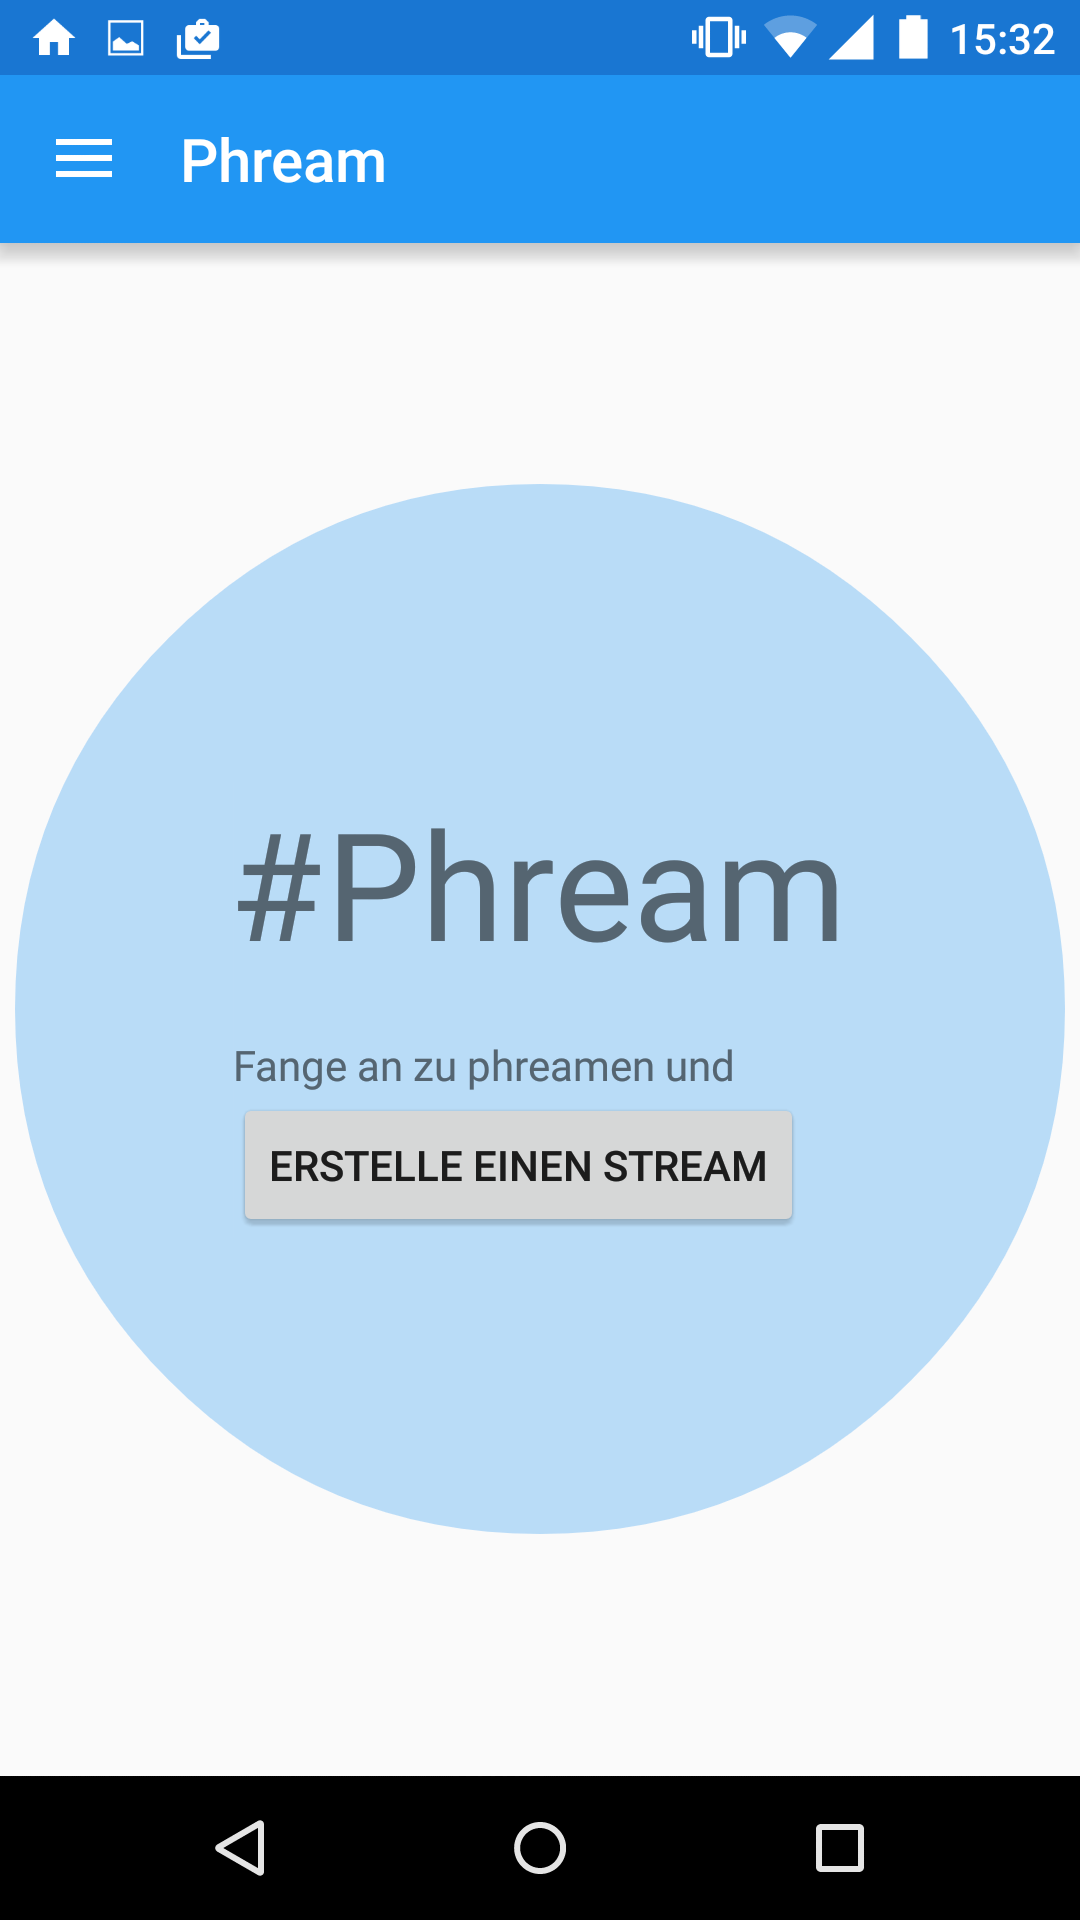
\includegraphics[width=0.6\textwidth]{images/screenshots/startview.png}
	\caption{App-Startansicht}
	\label{label:startview}
	\end{minipage}
	\hfill
	\begin{minipage}{0.4\textwidth}
	\centering
	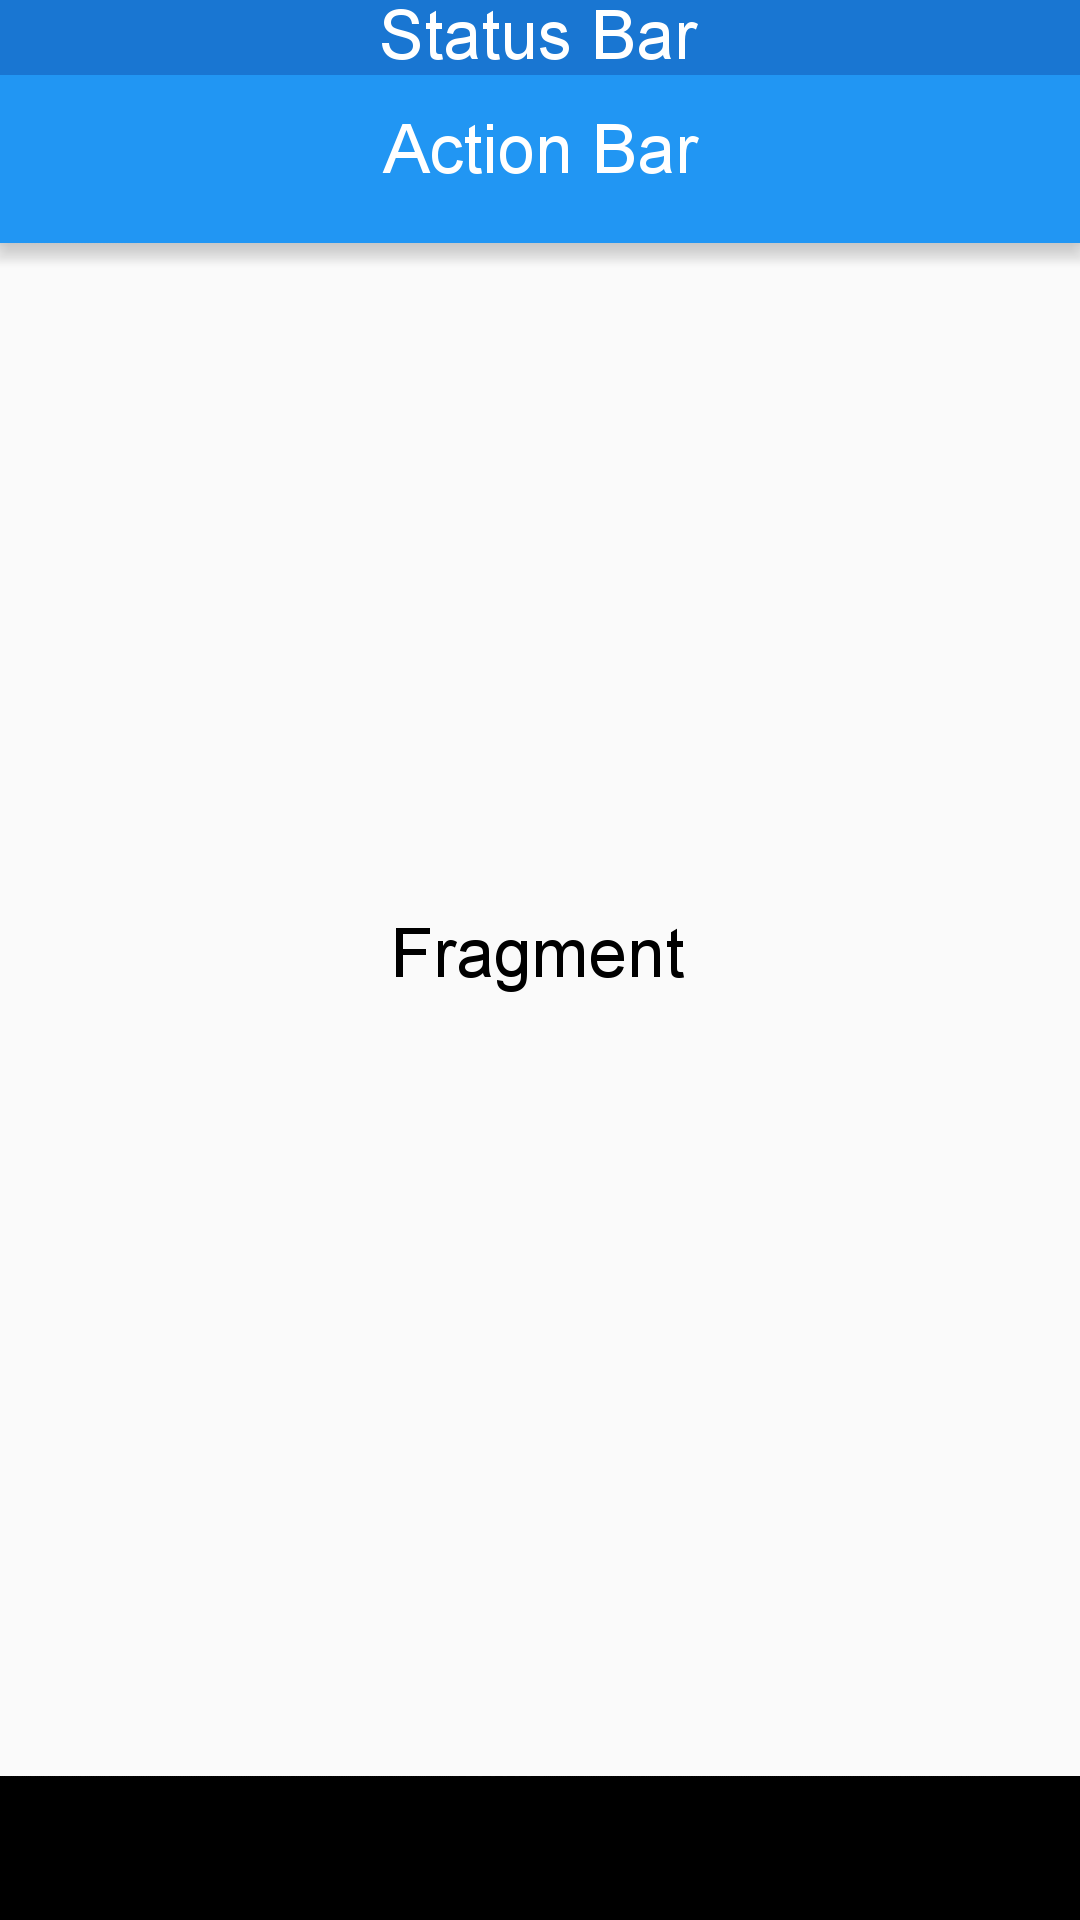
\includegraphics[width=0.6\textwidth]{images/screenshots/startview_schema.png}
	\caption{Schematische Darstellung}
	\label{label:startview_schema}
	\end{minipage}
\end{figure}
Die in Abbildung \ref{label:startview_schema} eingezeichnete Statusbar ist standardmäßig in jeder Ansicht der App zu sehen und zeigt allgemeine Statusinformationen zum Androidgerät an. Die Action Bar wird von der App selbst gestaltet und beinhaltet verschiedene Optionen, wie beispielsweise Menüs. Den größten Teil der App nimmt die Hauptansicht in Anspruch. In diesem werden die verschiedenen Informationen der App dargestellt. 

Die aktuelle Ansicht wird immer dann angezeigt, wenn noch kein Stream (Ordner) angelegt wurde. Durch anklicken des Buttons öffnet sich ein Eingabefenster, in dem ein neuer Streamname eingegeben werden kann. Nach Bestätigung des Streamnamens wird der Stream angelegt und erscheint daraufhin im Navigation Drawer. 

\subsection{Navigation Drawer}

Der Navigation Drawer (Abbildung \ref{label:navigationdrawer}) kann durch klicken auf das Menüicon oben links neben dem Titel oder durch einen Swipe vom linken Bildschirmrand geöffnet werden.
In der daraufhin eingeblendeten Ansicht hat der Benutzer die Möglichkeit zwischen verschiedenen Streams zu wechseln und neue Streams anzulegen. Durch anklicken eines Streamnamens wird dieser aktiv und wird daraufhin in der Hauptansicht angezeigt. Durch einen swipe zum linken Bildschirmrand oder durch anklicken des Pfeils links neben dem Appnamen kann der Navigation Drawer geschlossen werden.

\begin{figure}[H]
\centering
	\begin{minipage}{0.4\textwidth} 
	\centering
	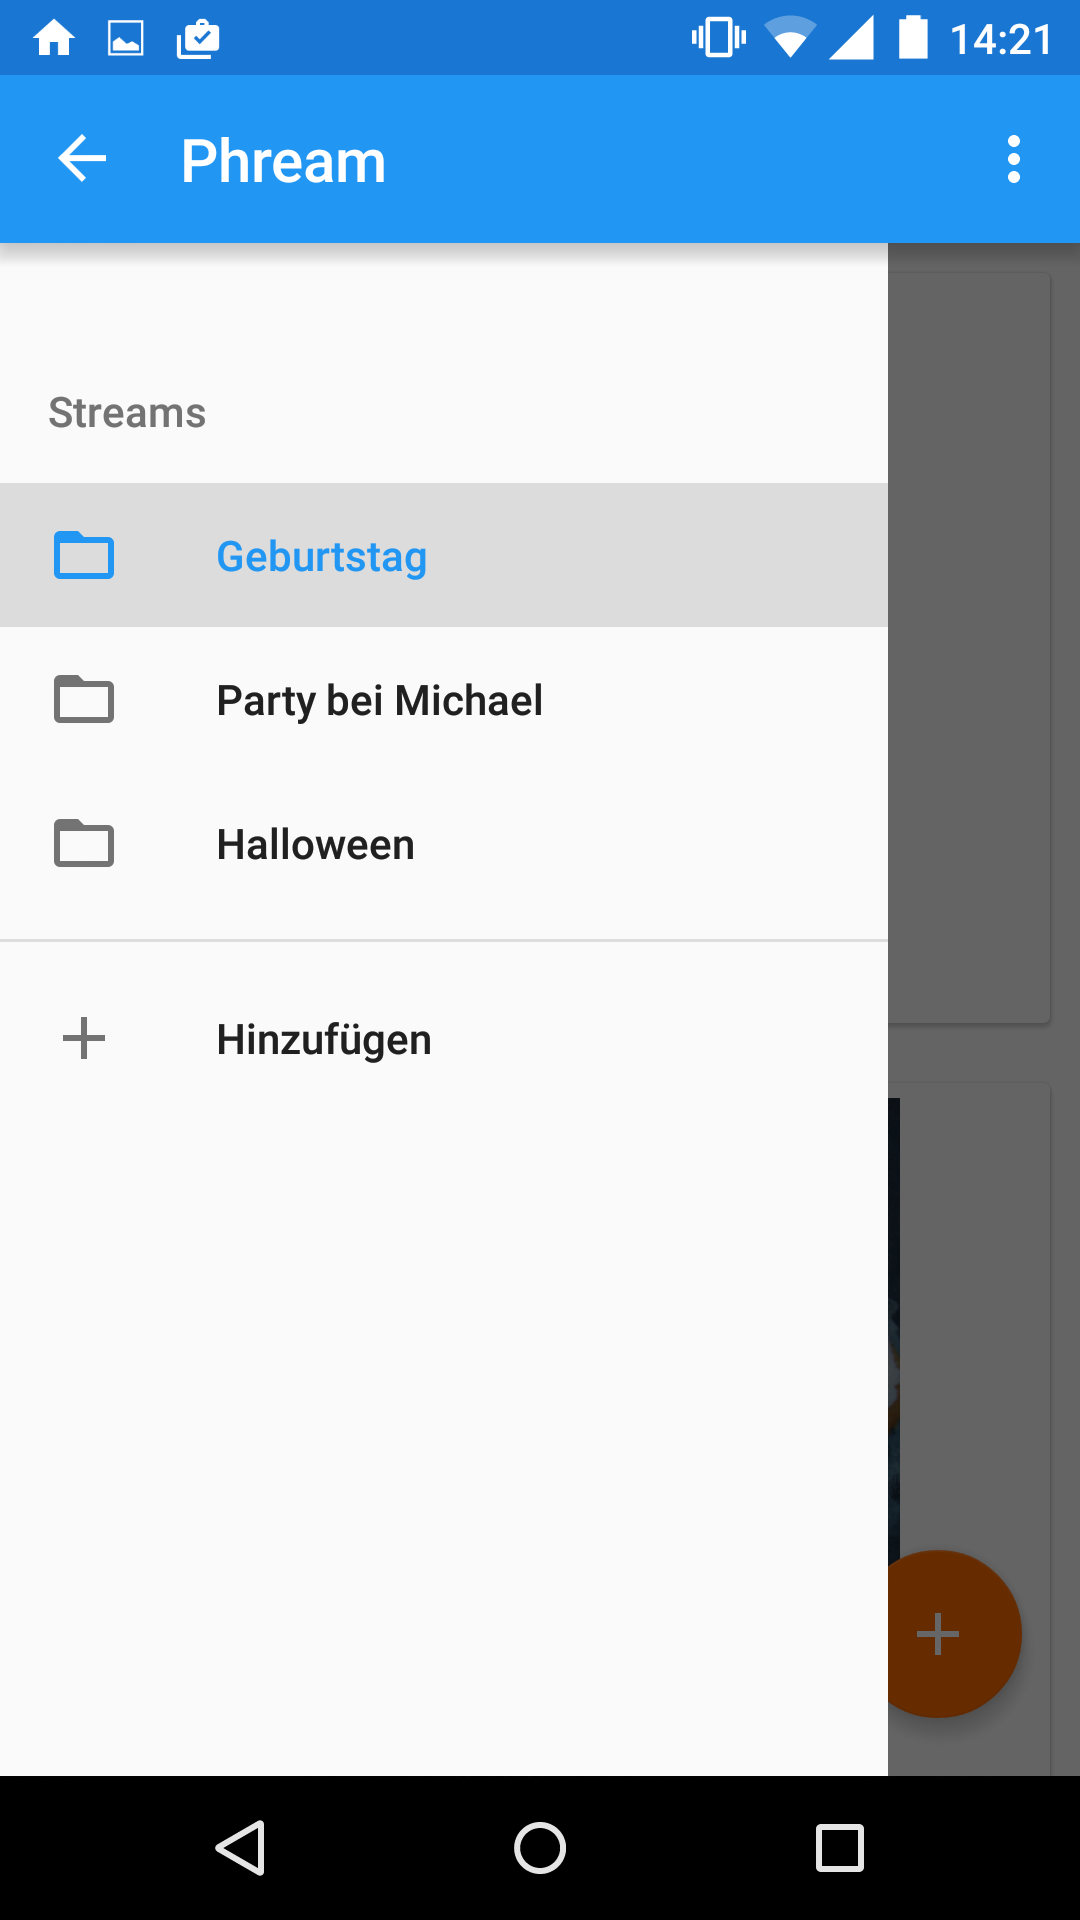
\includegraphics[width=0.6\textwidth]{images/screenshots/navigationdrawer.png}
	\caption{Navigation Drawer}
	\label{label:navigationdrawer}
	\end{minipage}
	%\hfill
	%\begin{minipage}{0.4\textwidth}
	%\centering
	%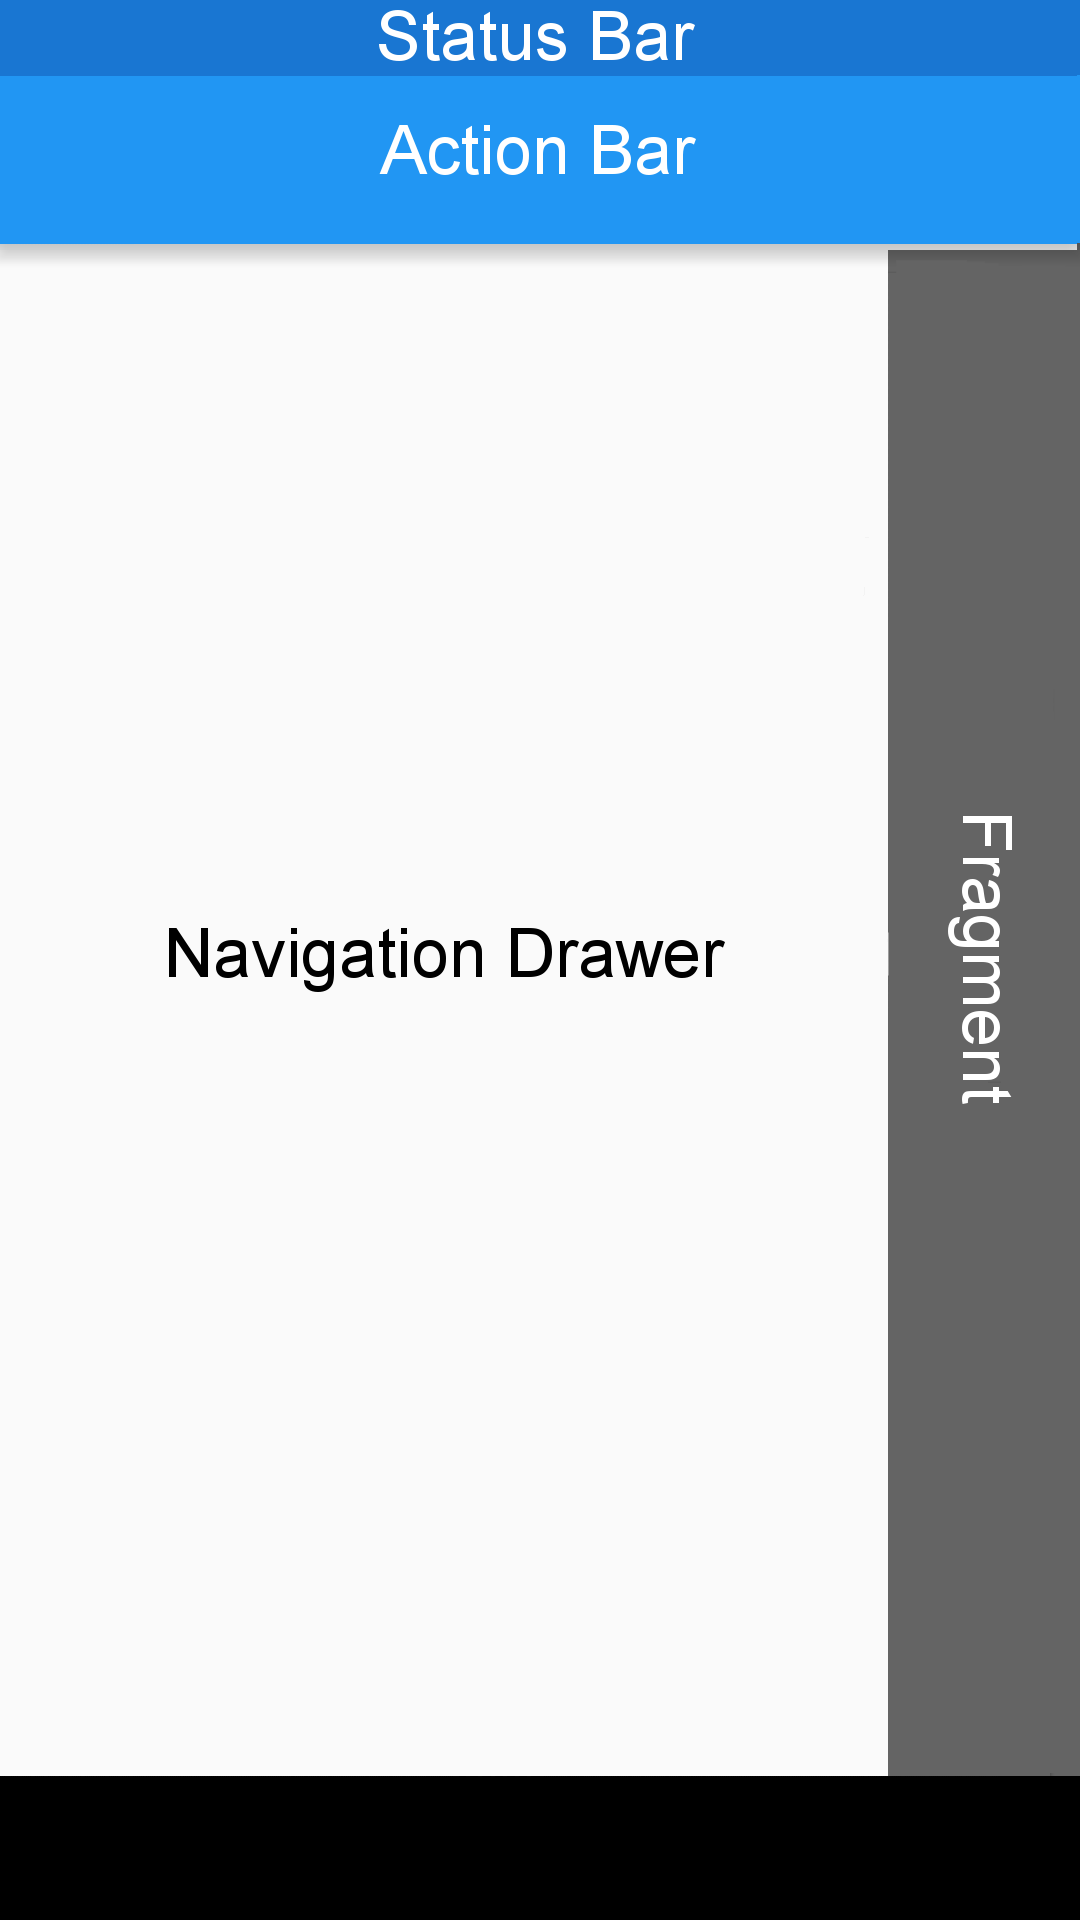
\includegraphics[width=0.6\textwidth]{images/screenshots/navigationdrawer_schema.png}
	%\caption{Schematische Darstellung}
	%\label{label:navigationdrawer_schema}
	%\end{minipage}
\end{figure}
%In der schematischen Darstellung (Abbildung \ref{label:navigationdrawer_schema}) ist zu sehen, dass der Navigation Drawer das aktuelle Fragment \enquote{überdeckt} und den restlichen Teil des Fragments abdunkelt. Der Navigation Drawer selbst wird dabei wieder aus einem Fragment zusammengesetzt. In der Action Bar wird dabei der Button zum Öffnen des Navigation Drawer zu einem Pfeil.

\subsection{Streamansicht}
Nach dem Auswählen eines Streams im Navigation Drawer (oder beim Appstart, wenn ein Stream angelegt ist) wird dieser in der Hauptansicht angezeigt. Die Streamansicht (Abbildung  \ref{label:streamview}) zeigt alle Bilder an, die dem entsprechenden Stream zugeordnet wurden. Die Hauptansicht wird dabei mit CardViews gefüllt, die eine ImageView mit einem Vorschaubild, dem Bildtitel, sowie Aufnahmeinformationen beinhalten. Der Benutzer kann durch Scroll-Gesten durch die Ansicht navigieren. Das oben rechts in der Action Bar angezeigte \enquote{Options-Symbol} beinhaltet die Optionen, den aktuellen Stream umzubenennen und zu löschen. Beim Löschvorgang eines Streams werden alle Daten zum Stream und dessen Inhalt aus der Datenbank und alle Bilder von der SD-Karte gelöscht.

\begin{figure}[H]
\centering
	\begin{minipage}{0.4\textwidth} 
	\centering
	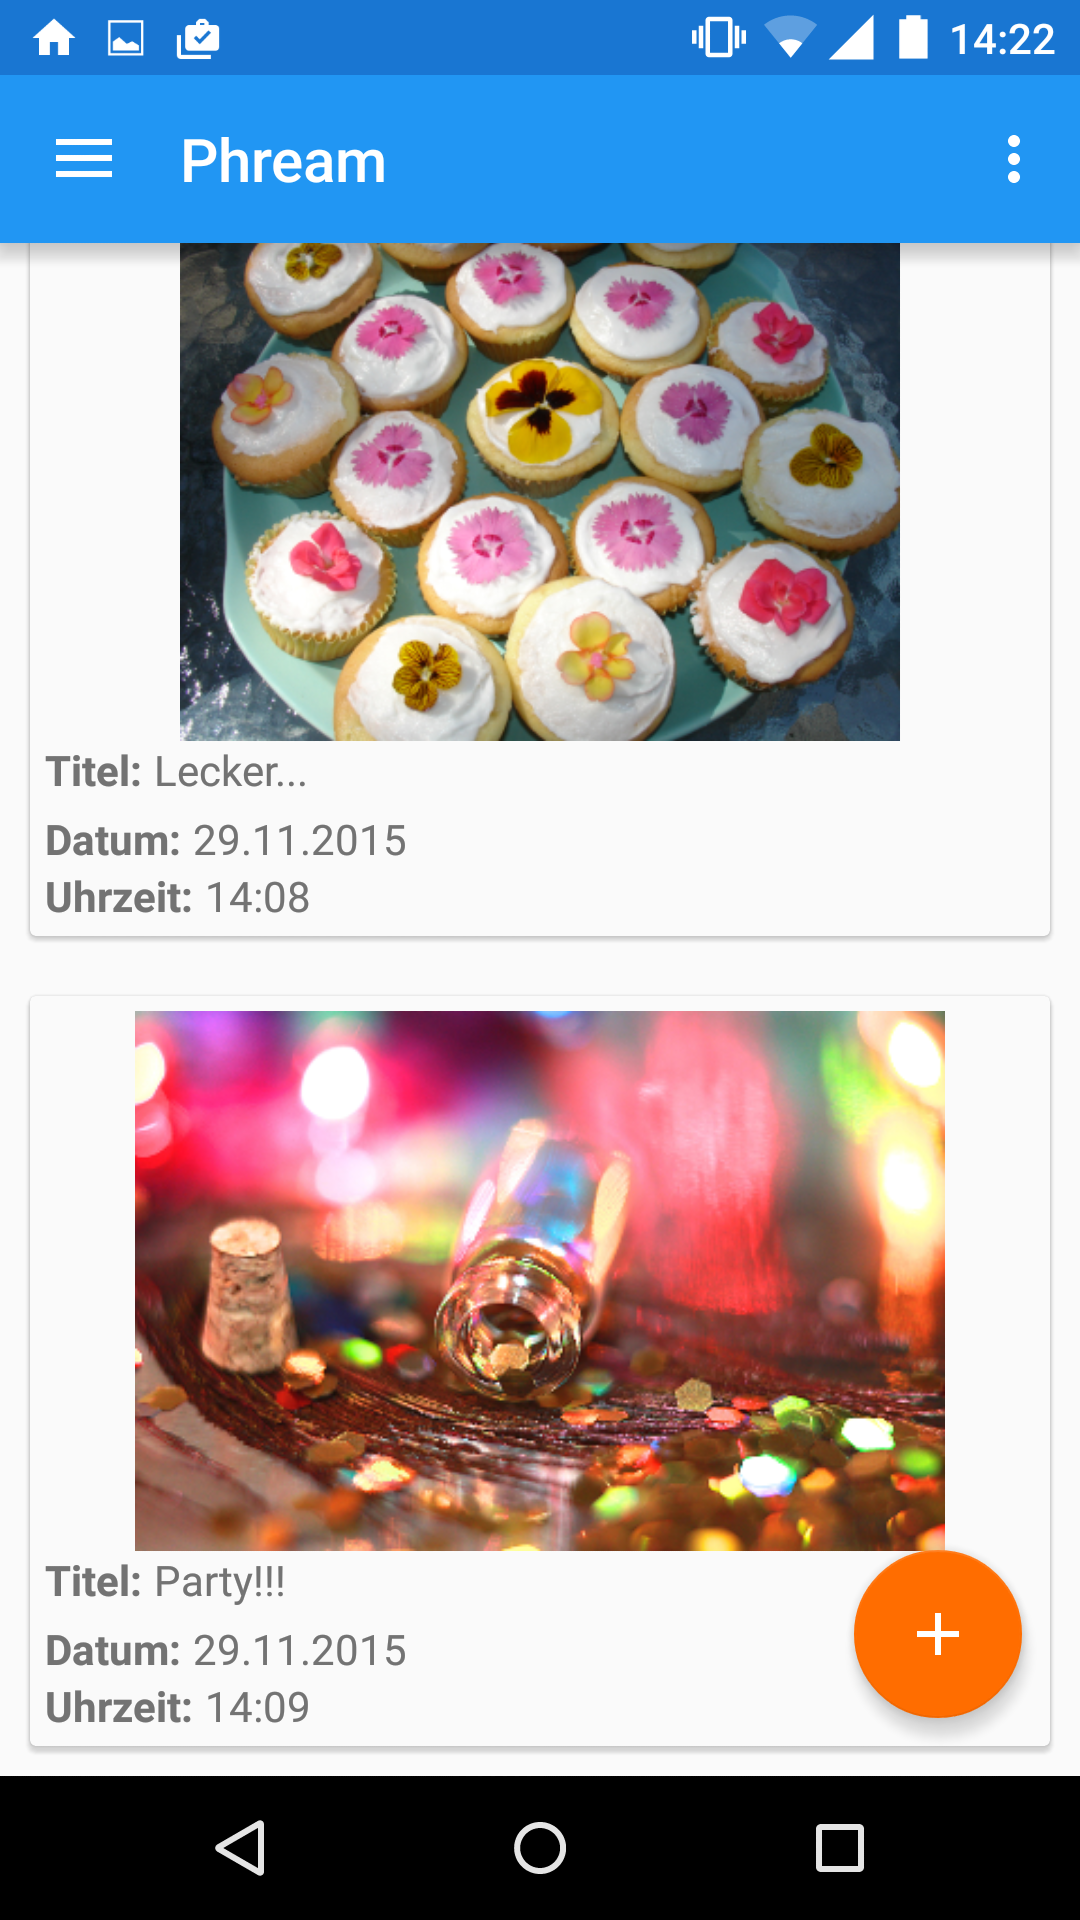
\includegraphics[width=0.6\textwidth]{images/screenshots/streamview.png}
	\caption{Streamansicht}
	\label{label:streamview}
	\end{minipage}
	\hfill
	\begin{minipage}{0.4\textwidth}
	\centering
	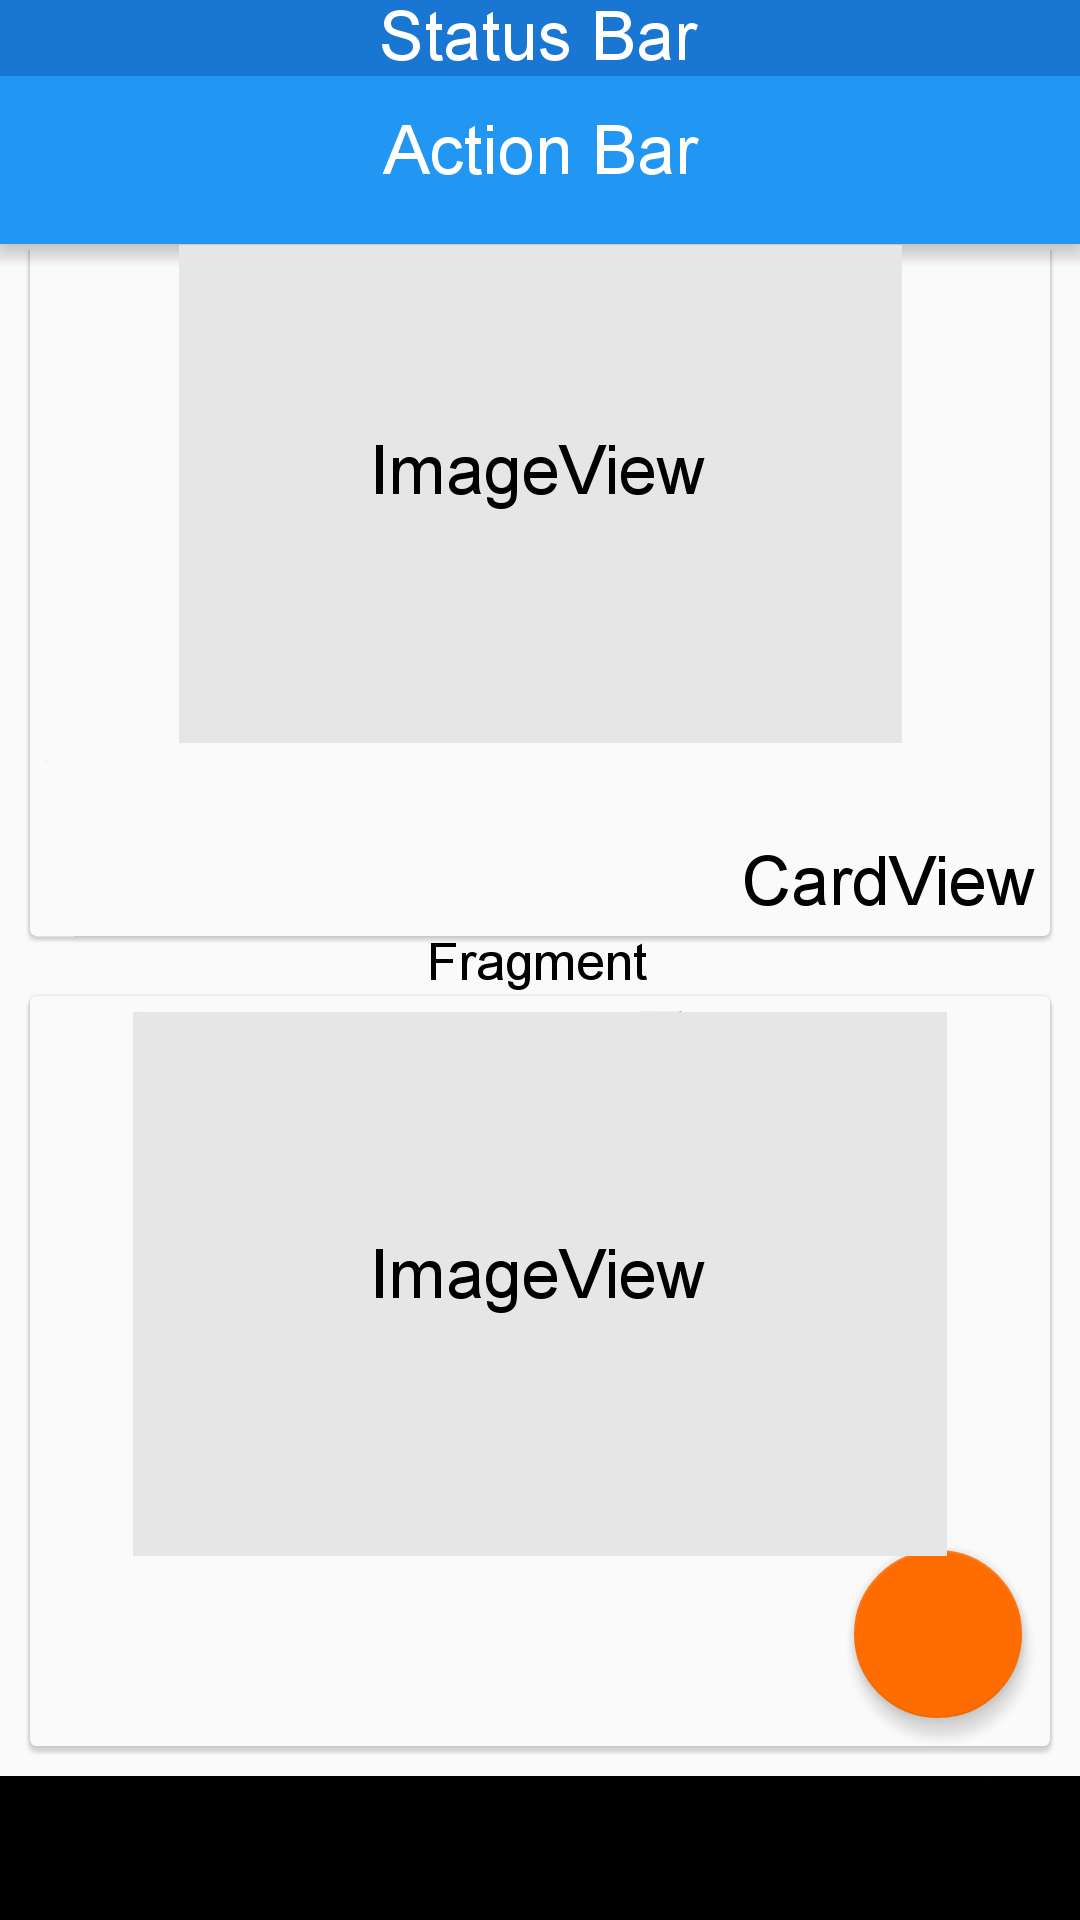
\includegraphics[width=0.6\textwidth]{images/screenshots/streamview_schema.png}
	\caption{Schematische Darstellung}
	\label{label:streamview_schema}
	\end{minipage}
\end{figure}

\subsubsection{Kontextmenü des CardView}

Durch einen \enquote{long tap} auf eine CardView in der Hauptansicht öffnet sich ein Kontextmenü zum aktuellen Bild. Das Kontextmenü bietet verschiedene Optionen, wie das Umbenennen des Bildes, das Löschen des Bildes und eine Möglichkeit zum Export in die Galerie. 
% Durch antippen der gewünschten Option erscheinen zusätzliche Abfragen je nach Menüeintrag. Es wird beispielsweise beim Umbenennen ein AlertDialog erzeugt, der die Eingabe eines neuen Bildtitels ermöglicht. Beim Löschen oder Exportieren des Bildes sollen eingeblendete AlertDialogs versehentliche Nutzeraktionen abfangen und eine Bestätigung der Aktion vom Benutzer erfragen.

\begin{figure}[H]
	\centering
   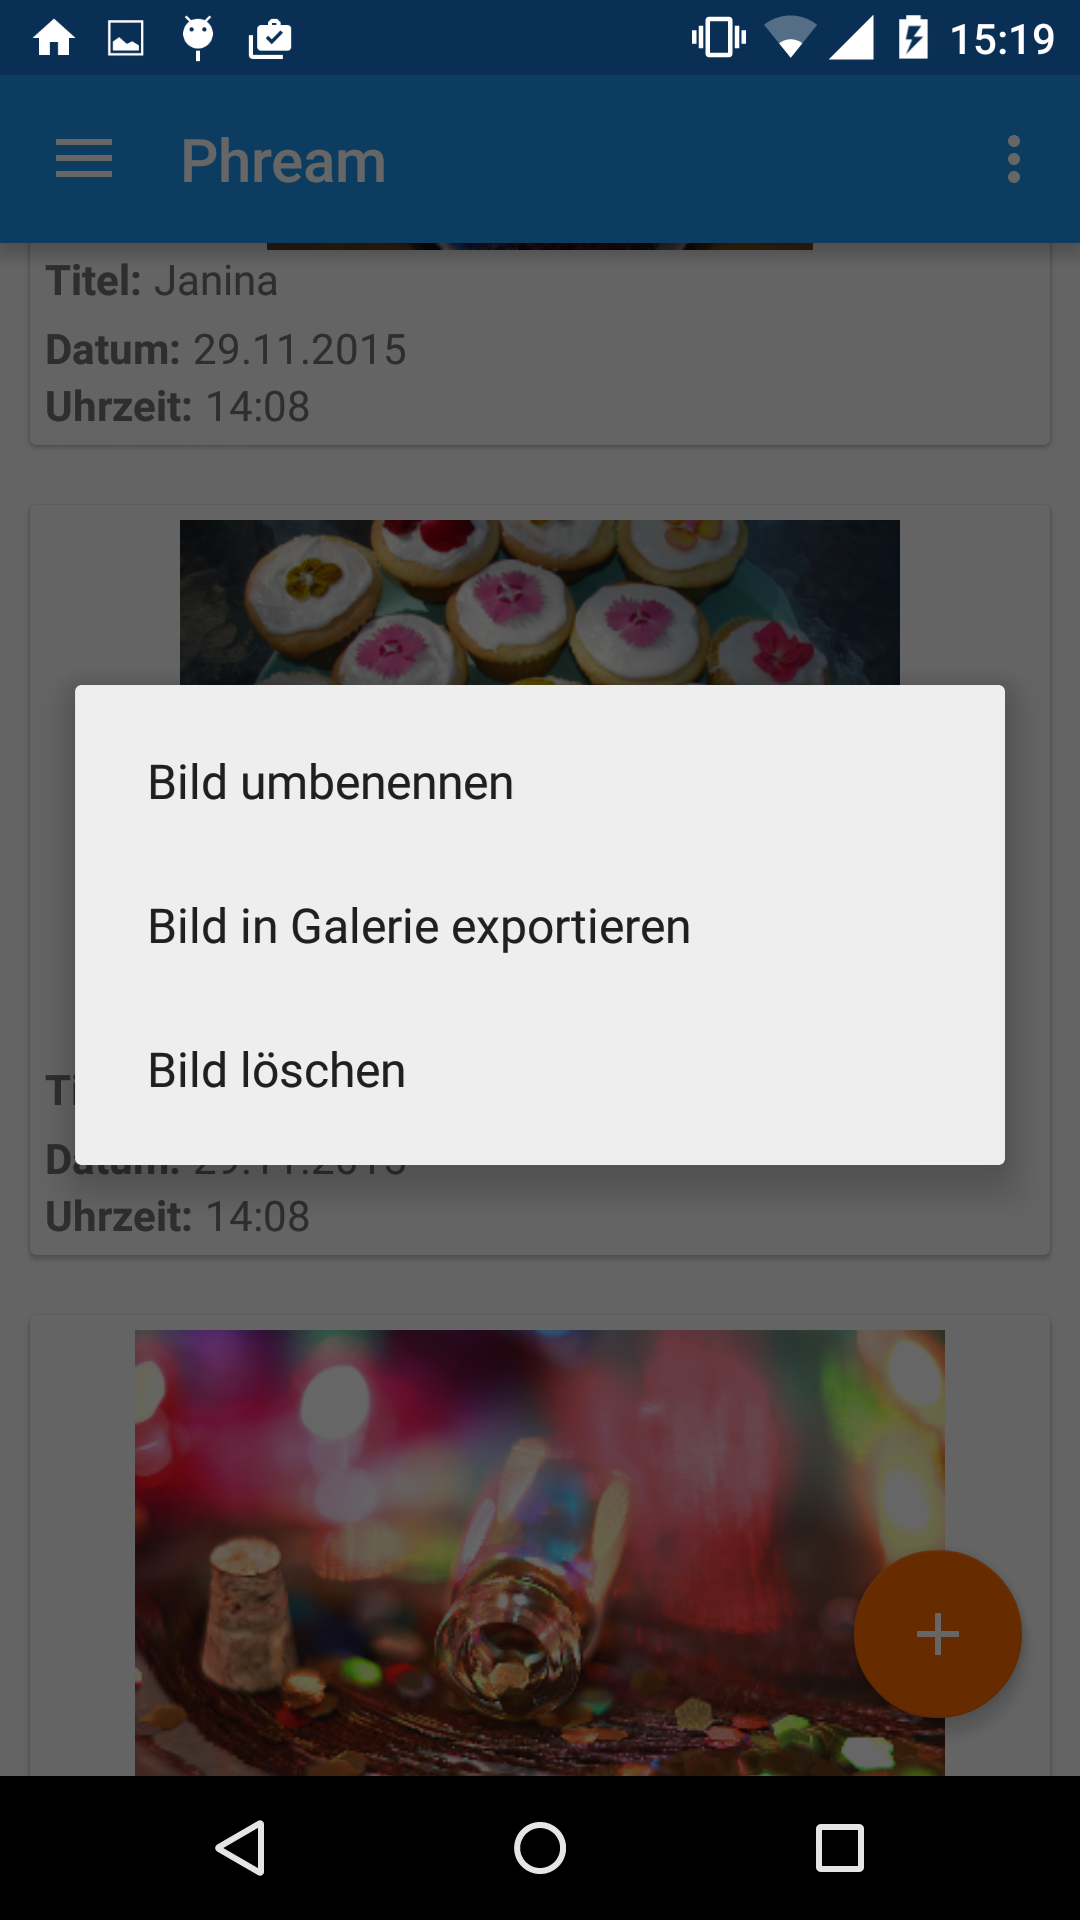
\includegraphics[scale= 0.115]{images/screenshots/contextmenu.png}
  \caption{Kontextmenü - CardView}
\end{figure}

\section{Detailansicht eines Bildes}
Durch anklicken einer Card in der Hauptansicht, öffnet sich eine zweite Activity die eine Detailansicht (Abbildung \ref{label:fullscreenview}) des Bildes im Vollbild ermöglicht. Die Detailansicht besteht dabei aus einer Fullscreenactivity mit einer ImageView, die die gesamte Activity ausfüllt.
\begin{figure}[H]
\centering
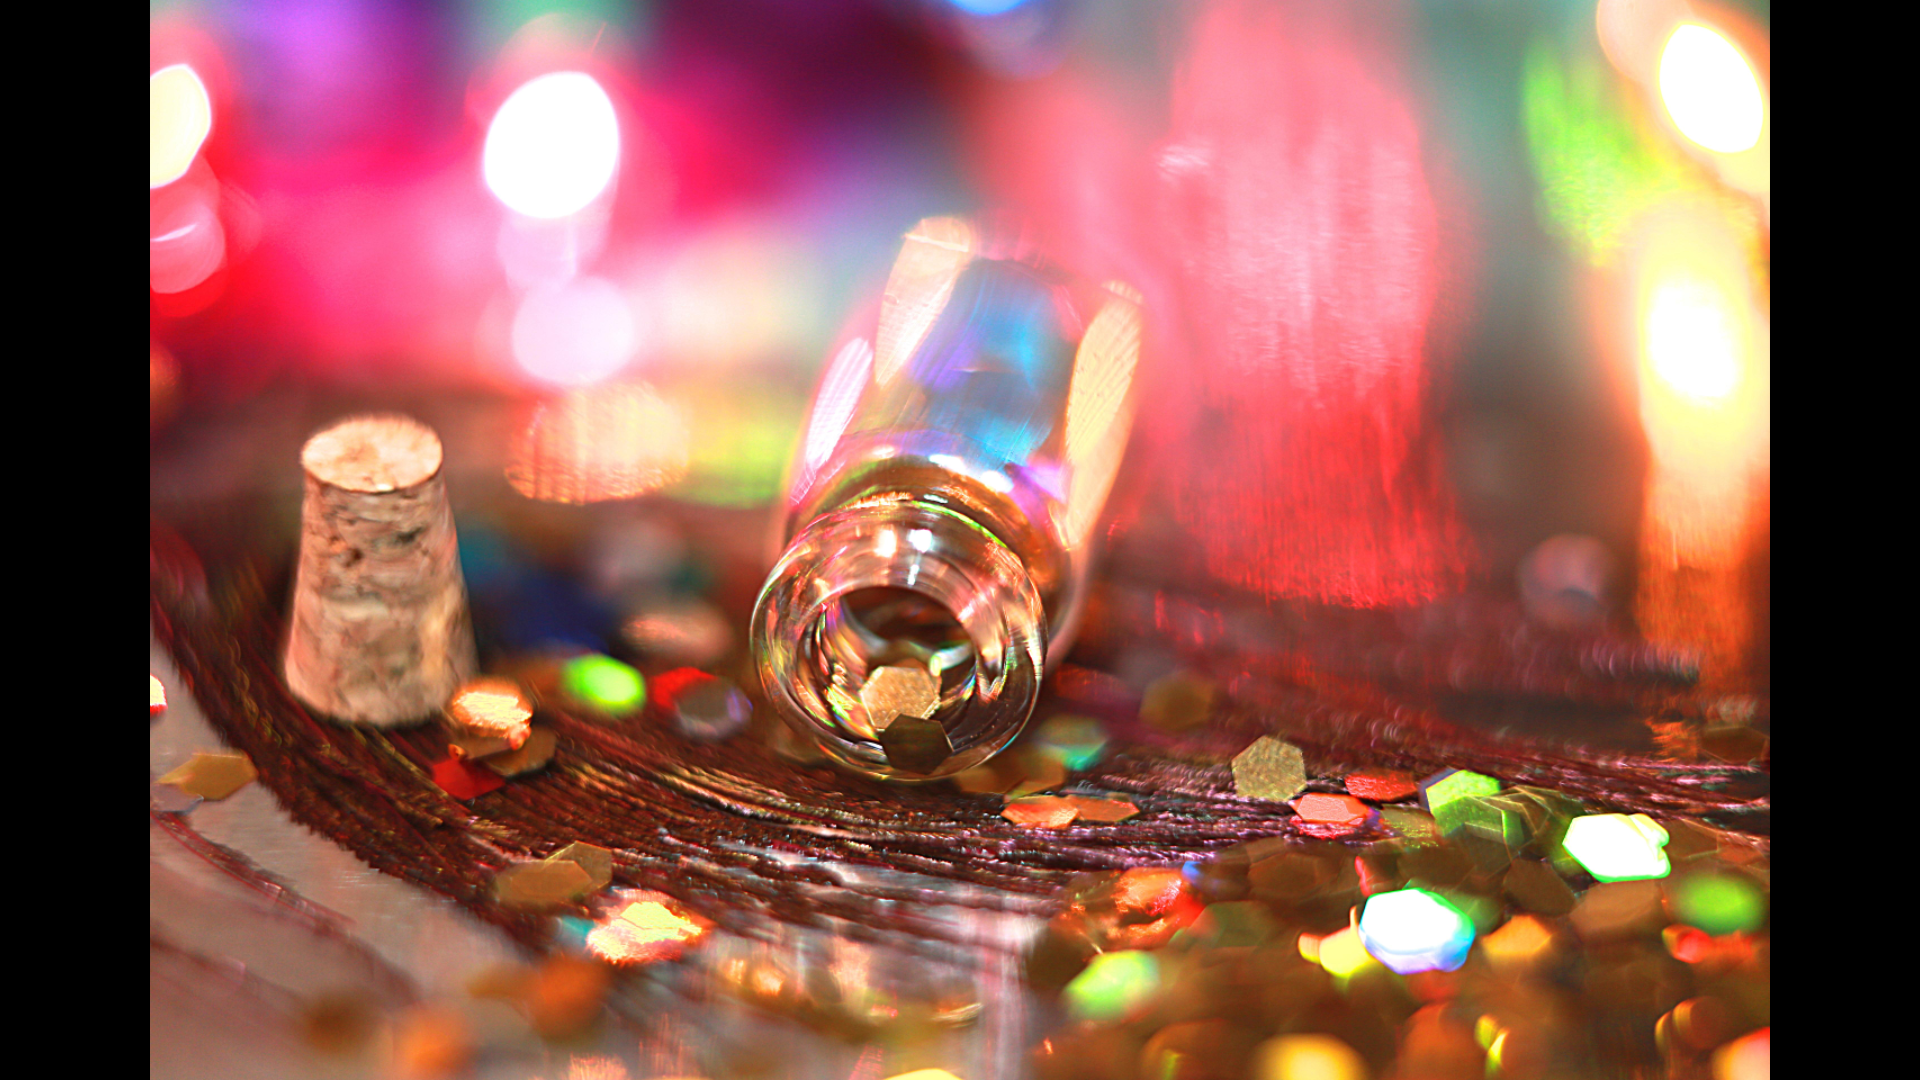
\includegraphics[scale=0.09]{images/screenshots/fullscreenview.png}
\caption{Detailansicht eines Bildes}
\label{label:fullscreenview}
\end{figure}

Durch einen \enquote{short tap} wird die Status Bar und die Action Bar wieder eingeblendet und bietet dem Bentuzer verschiedene Interaktionsmöglichkeiten (Abbildung \ref{label:fullscreenview_menu}).

\begin{figure}[H]
\centering
	\begin{minipage}{0.4\textwidth} 
	\centering
	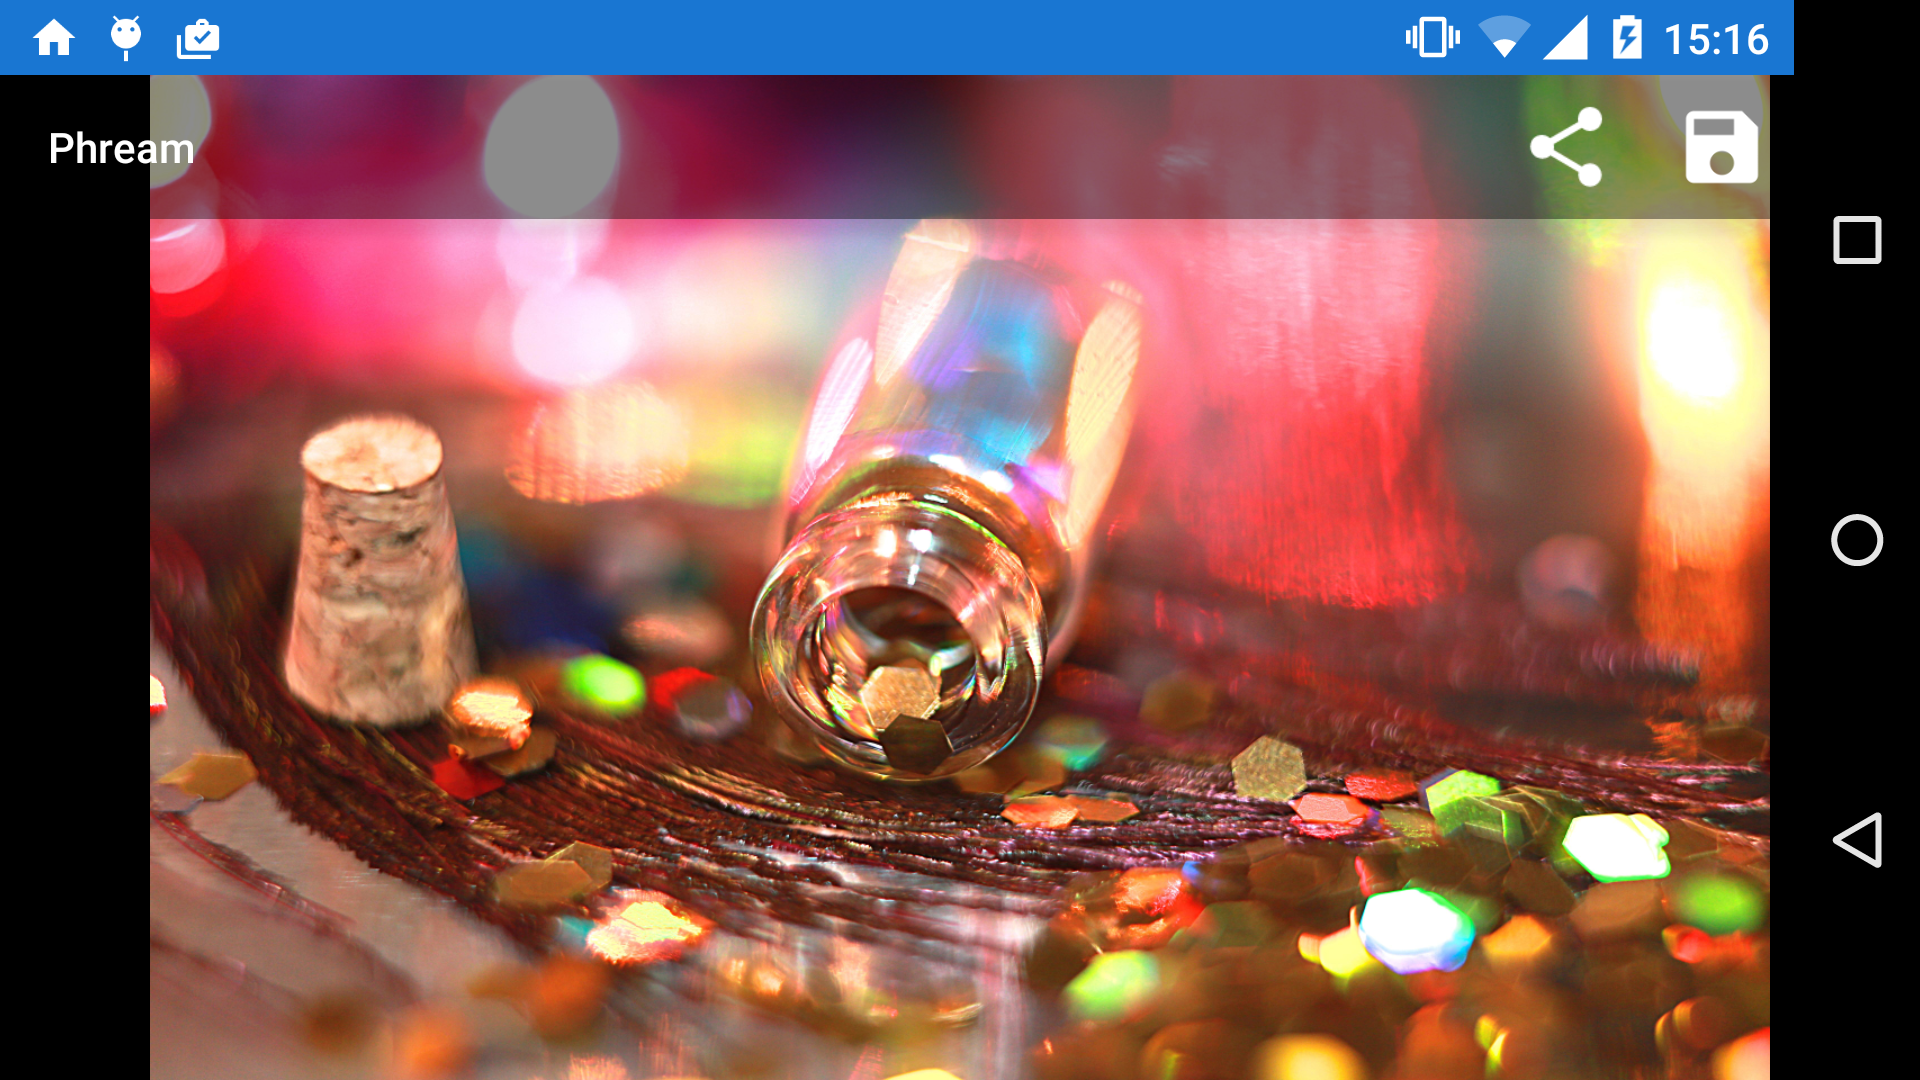
\includegraphics[width=1\textwidth]{images/screenshots/fullscreenview_menu.png}
	\caption{Detailansicht mit Action Bar}
	\label{label:fullscreenview_menu}
	\end{minipage}
	\hfill
	\begin{minipage}{0.4\textwidth}
	\centering
	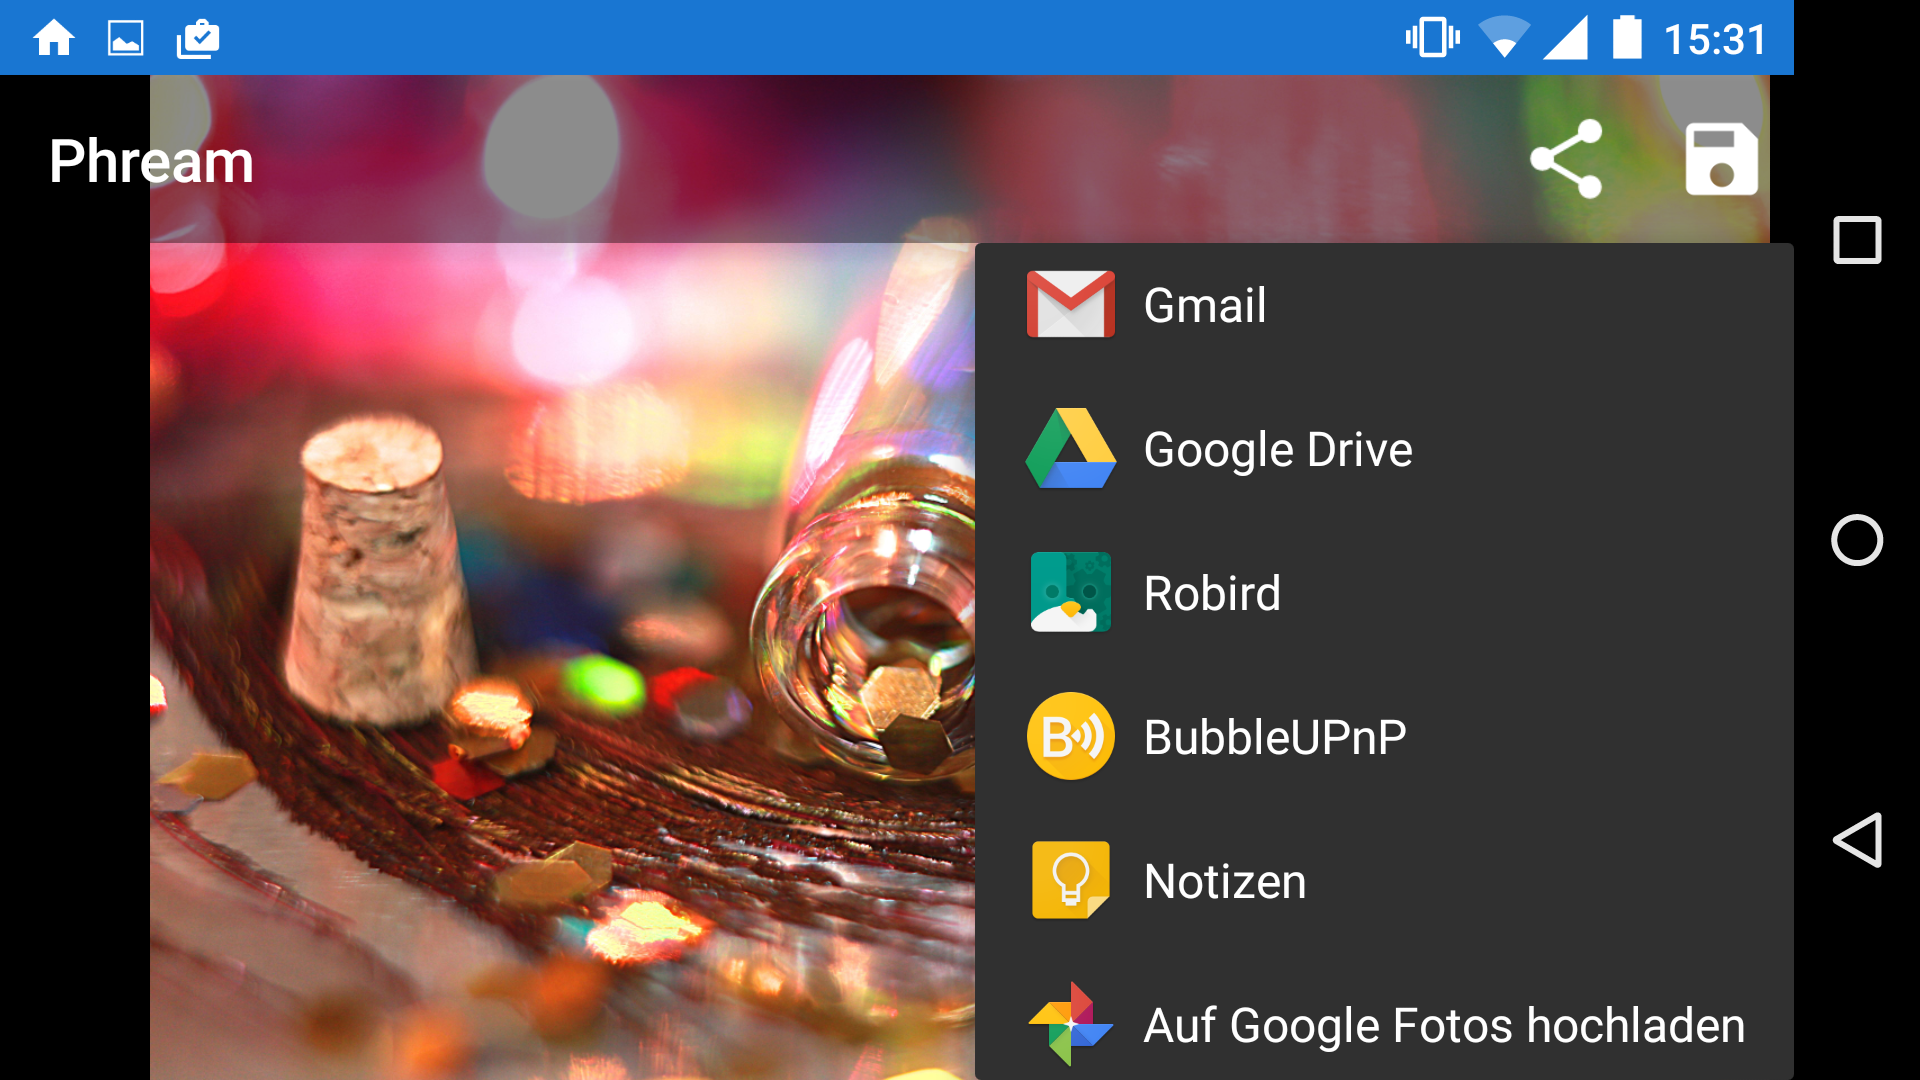
\includegraphics[width=1\textwidth]{images/screenshots/fullscreenview_share.png}
	\caption{Share-Provider}
	\label{label:fullscreenview_share}
	\end{minipage}
\end{figure}

Durch anklicken des \enquote{Speichern-Symbols} oben rechts in der Action Bar kann der Benutzer das aktuelle Bild in die Android Galerie exportieren. Dieses wird daraufhin mit aktuellen Datum und Uhrzeit als erstes in der Android Galerie angezeit. Durch antippen des \enquote{Share-Symbols} öffnet sich der Share Provider (Abbildung \ref{label:fullscreenview_share}) von Android. Der Share-Provider ist ein allgemeines Framework, welches die Option bietet verschiedene Dateien mit anderen Apps zu teilen oder ihnen zur Verfügung zu stellen. Eine Option ist beispielsweise, sofern ein E-Mail Client vorhanden ist, das aktuelle Bild per E-Mail zu versenden.

\section{Der Floating Action Button}
Der Floating Action Button in der Hauptansicht dient der Gruppierung zweier wichtiger Funktionen der App. Dabei öffnet der Floating Action Button durch antippen ein Menu mit weiteren Optionen (Abbildung \ref{label:floatingaction_menu}). Weiterhin ist der Floating Action Button leicht durch eine Daumengeste erreichbar und gruppiert die Hauptfunktionalitäten der aktuellen Activity in einem Punkt. Je nach angetippten Menüeintrag startet der Galerieimport oder ein Kamera-Intent zum Aufnehmen eines Fotos.

\begin{figure}[H]
\centering
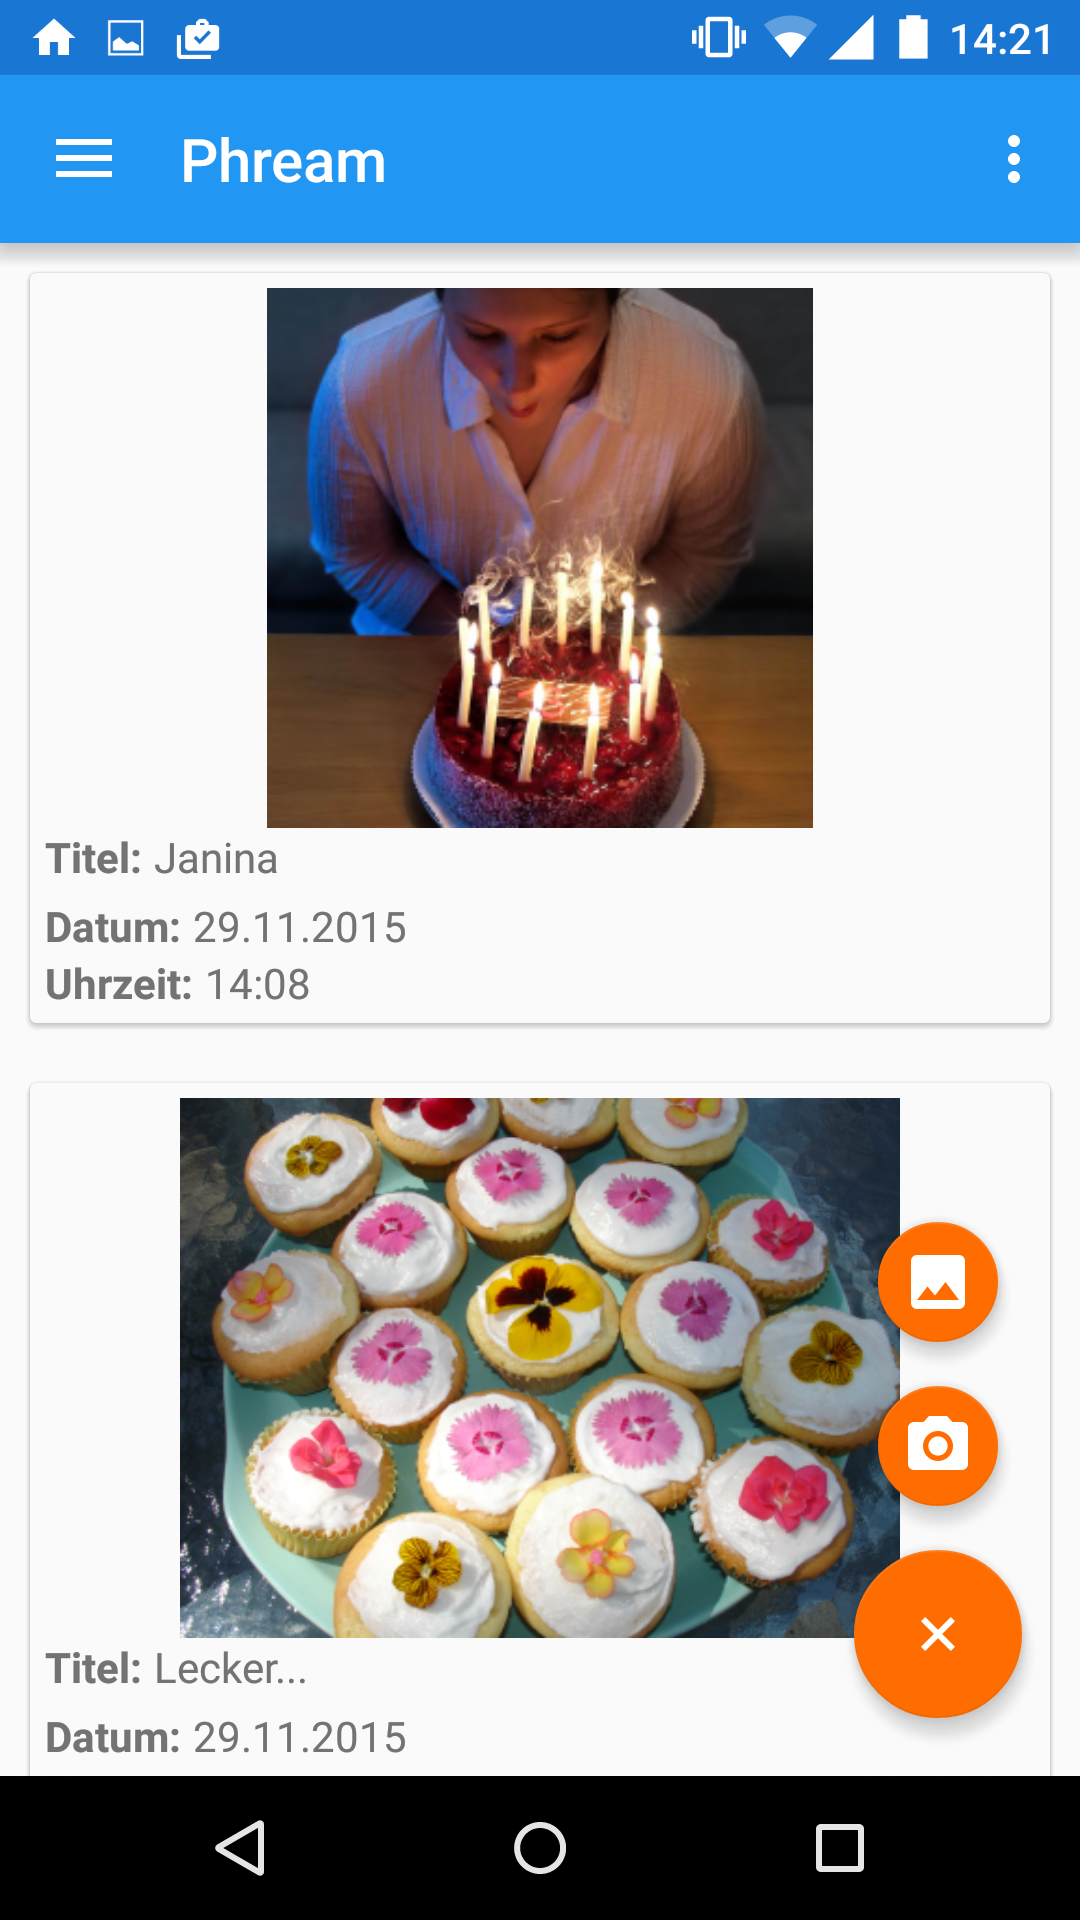
\includegraphics[scale=0.1]{images/screenshots/floatingaction_menu.png}
\caption{Floating Action Menu}
\label{label:floatingaction_menu}
\end{figure}

\subsection{Aufnehmen eines Fotos}
Nach dem Auswählen des Menü Eintrags im Floating Action Menu startet ein Kamera-Intent (Abbildung \ref{label:camera}), über das der Benutzer ein Foto aufnehmen kann und auch alle weiteren Kameraoptionen zur Verfügung hat. Nach dem Bestätigen des aufgenommenen Fotos kann der Benutzer einen Bildtitel (Abbildung \ref{label:camera_imagetitle}) festlegen.
\begin{figure}[H]
\centering
	\begin{minipage}{0.4\textwidth} 
	\centering
	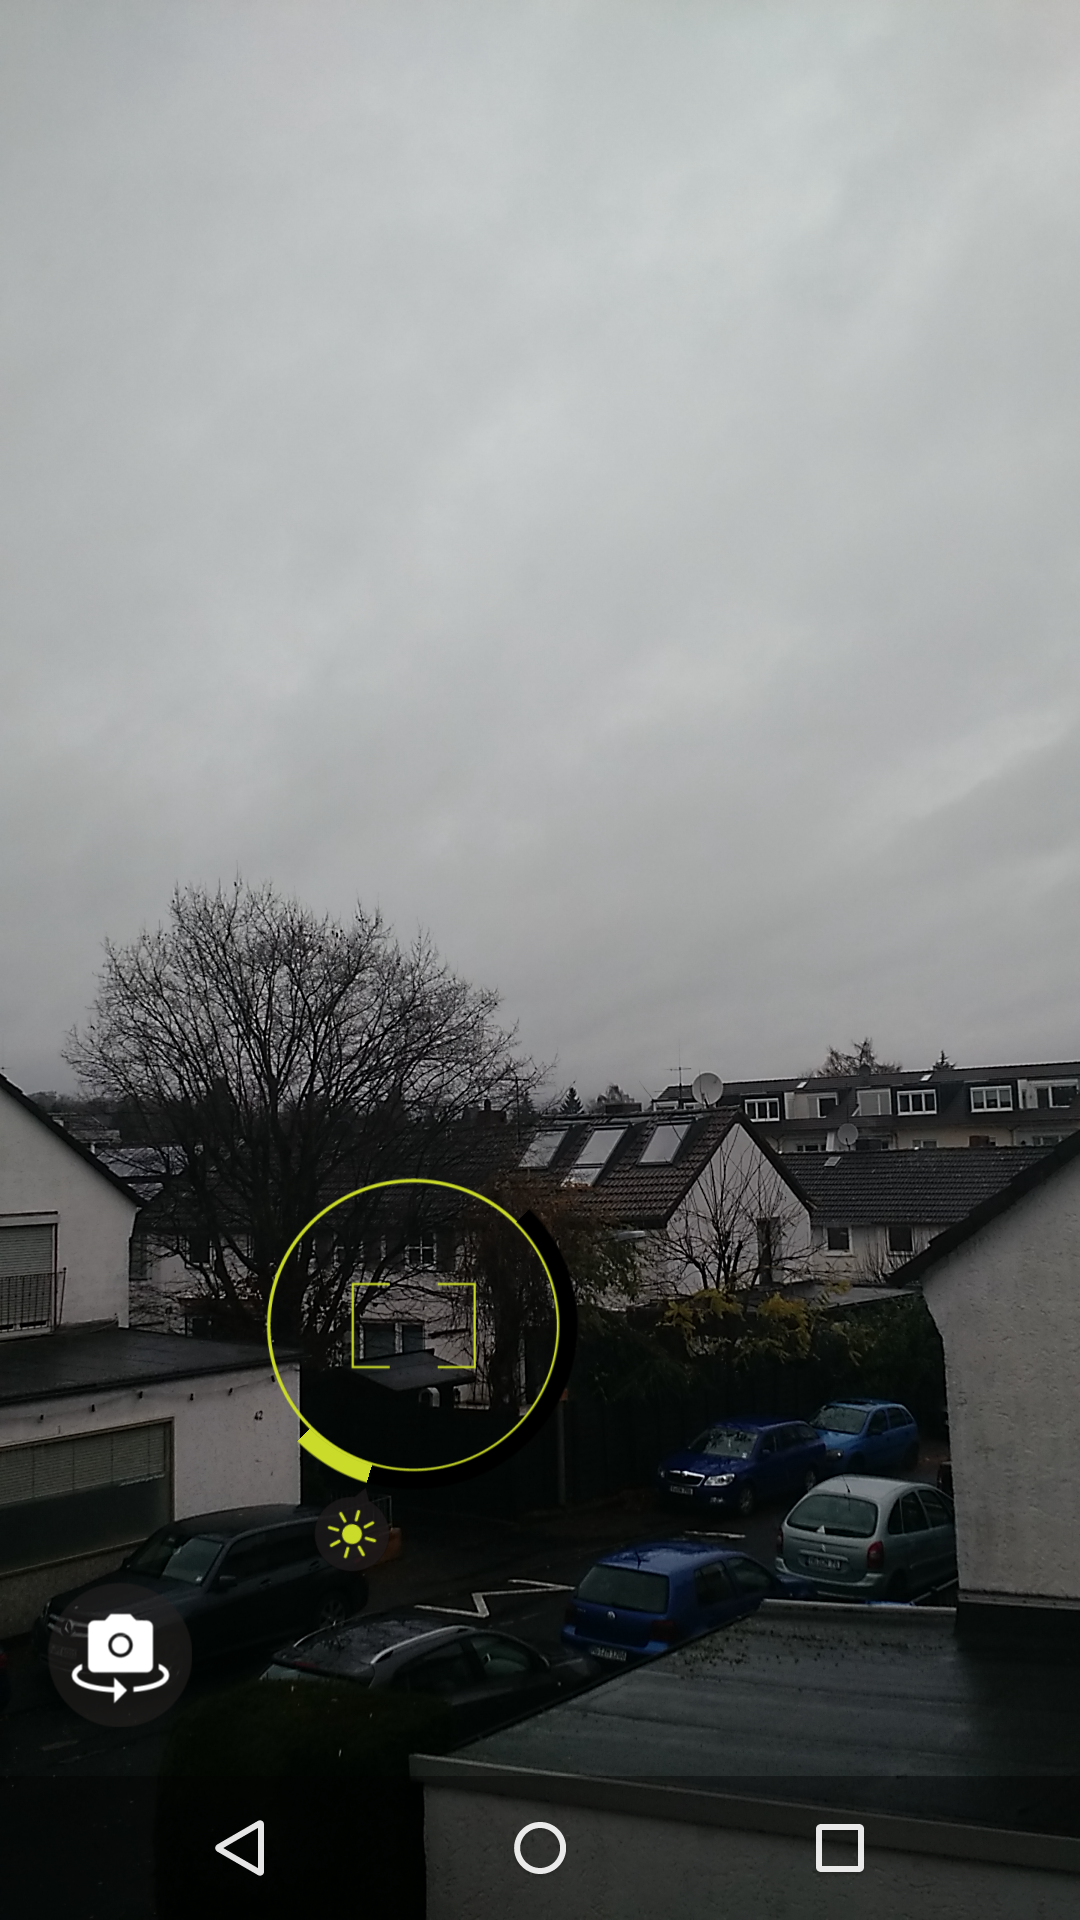
\includegraphics[width=0.6\textwidth]{images/screenshots/camera.png}
	\caption{Kamera-Intent}
	\label{label:camera}
	\end{minipage}
	\hfill
	\begin{minipage}{0.4\textwidth}
	\centering
	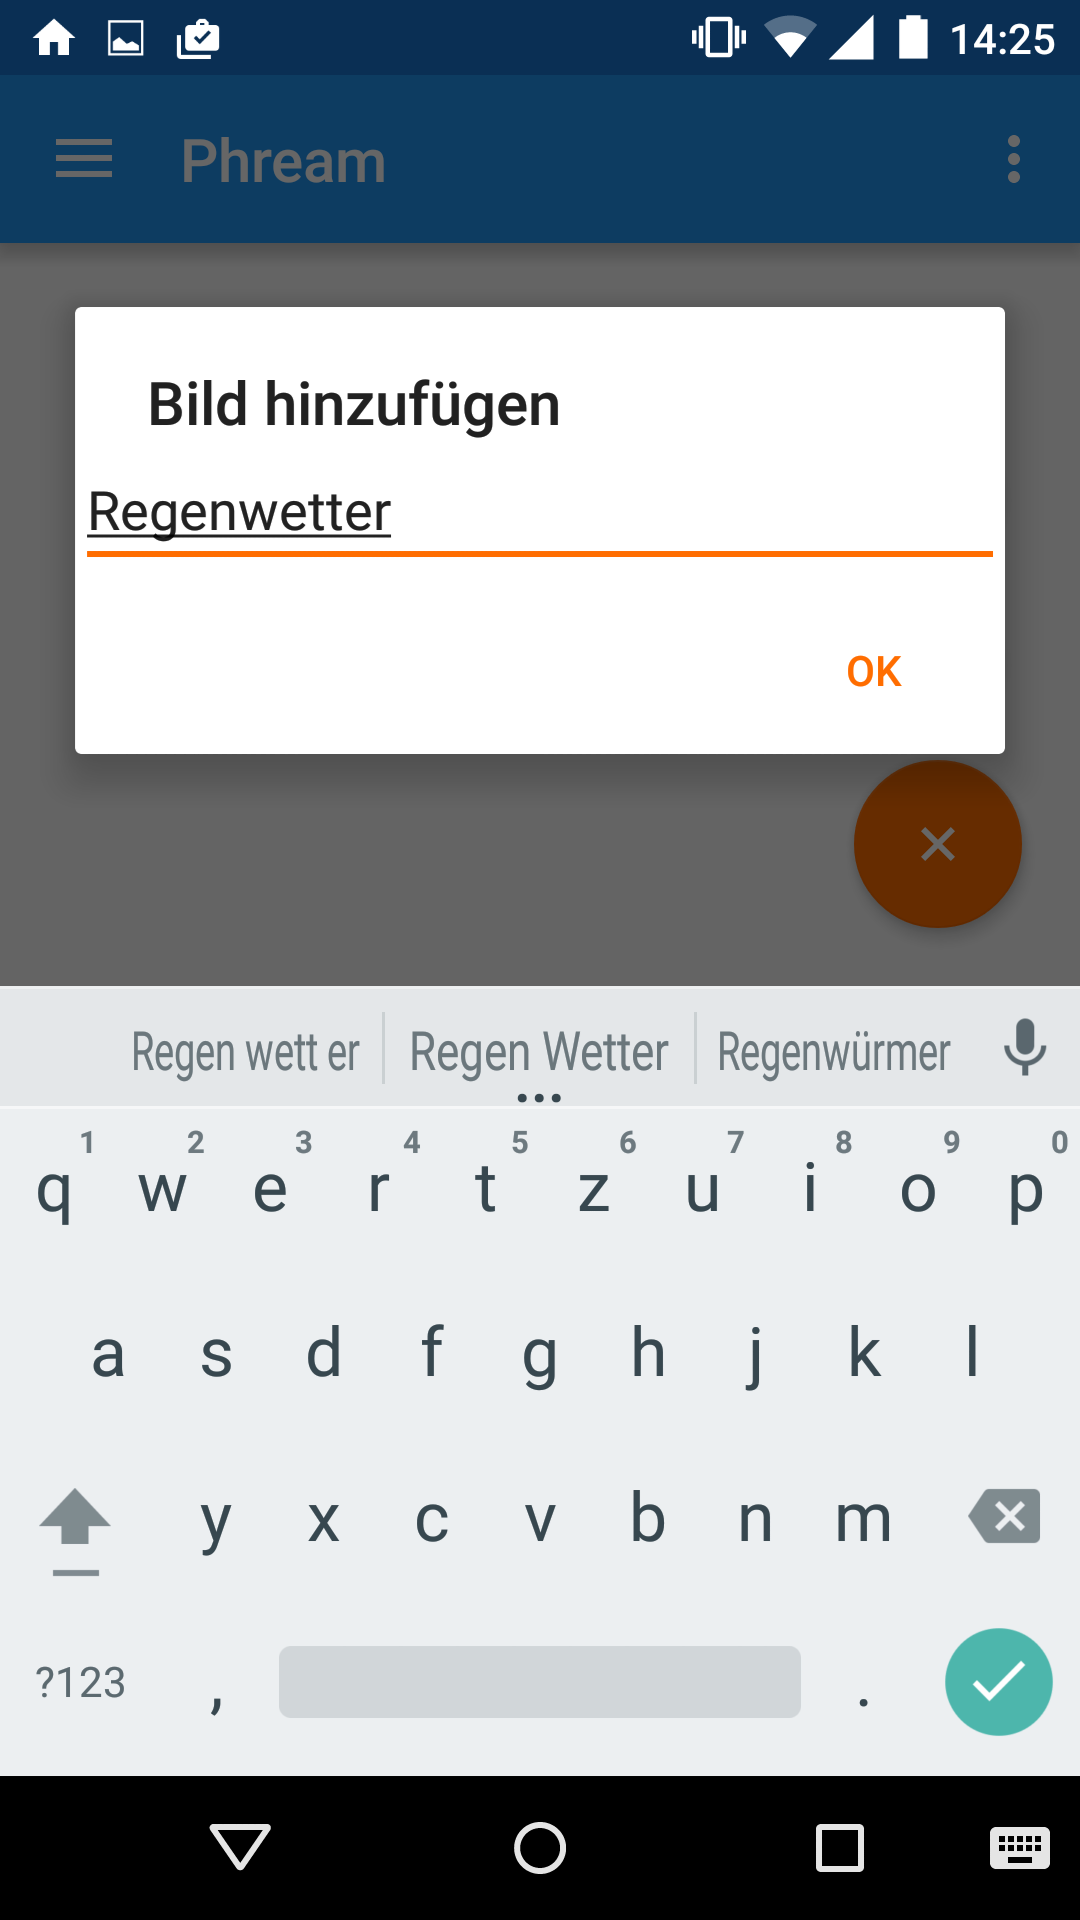
\includegraphics[width=0.6\textwidth]{images/screenshots/camera_imagetitle.png}
	\caption{Bildtitel festlegen}
	\label{label:camera_imagetitle}
	\end{minipage}
\end{figure}

\subsection{Importieren eines Fotos}
Nach dem Auswählen der Importierfunktion im Floating Action Menu startet der Content-Provider (Abbildung \ref{label:content_provider}), der dem Benutzer die Option bietet Dateien (in diesem Fall Bilder) auszuwählen. Dabei beschränkt sich die Dateiauswahl nicht nur auf die eigene Galerie, sondern zeigt auch, falls vorhanden, Bilder aus Google Drive oder Dropbox an. Dabei werden die Bilder erst aus der Cloud geladen und dann in die App importiert. Nach dem Importieren des Bildes kann der Benutzer wieder einen Bildtitel festlegen.

\begin{figure}[H]
\centering
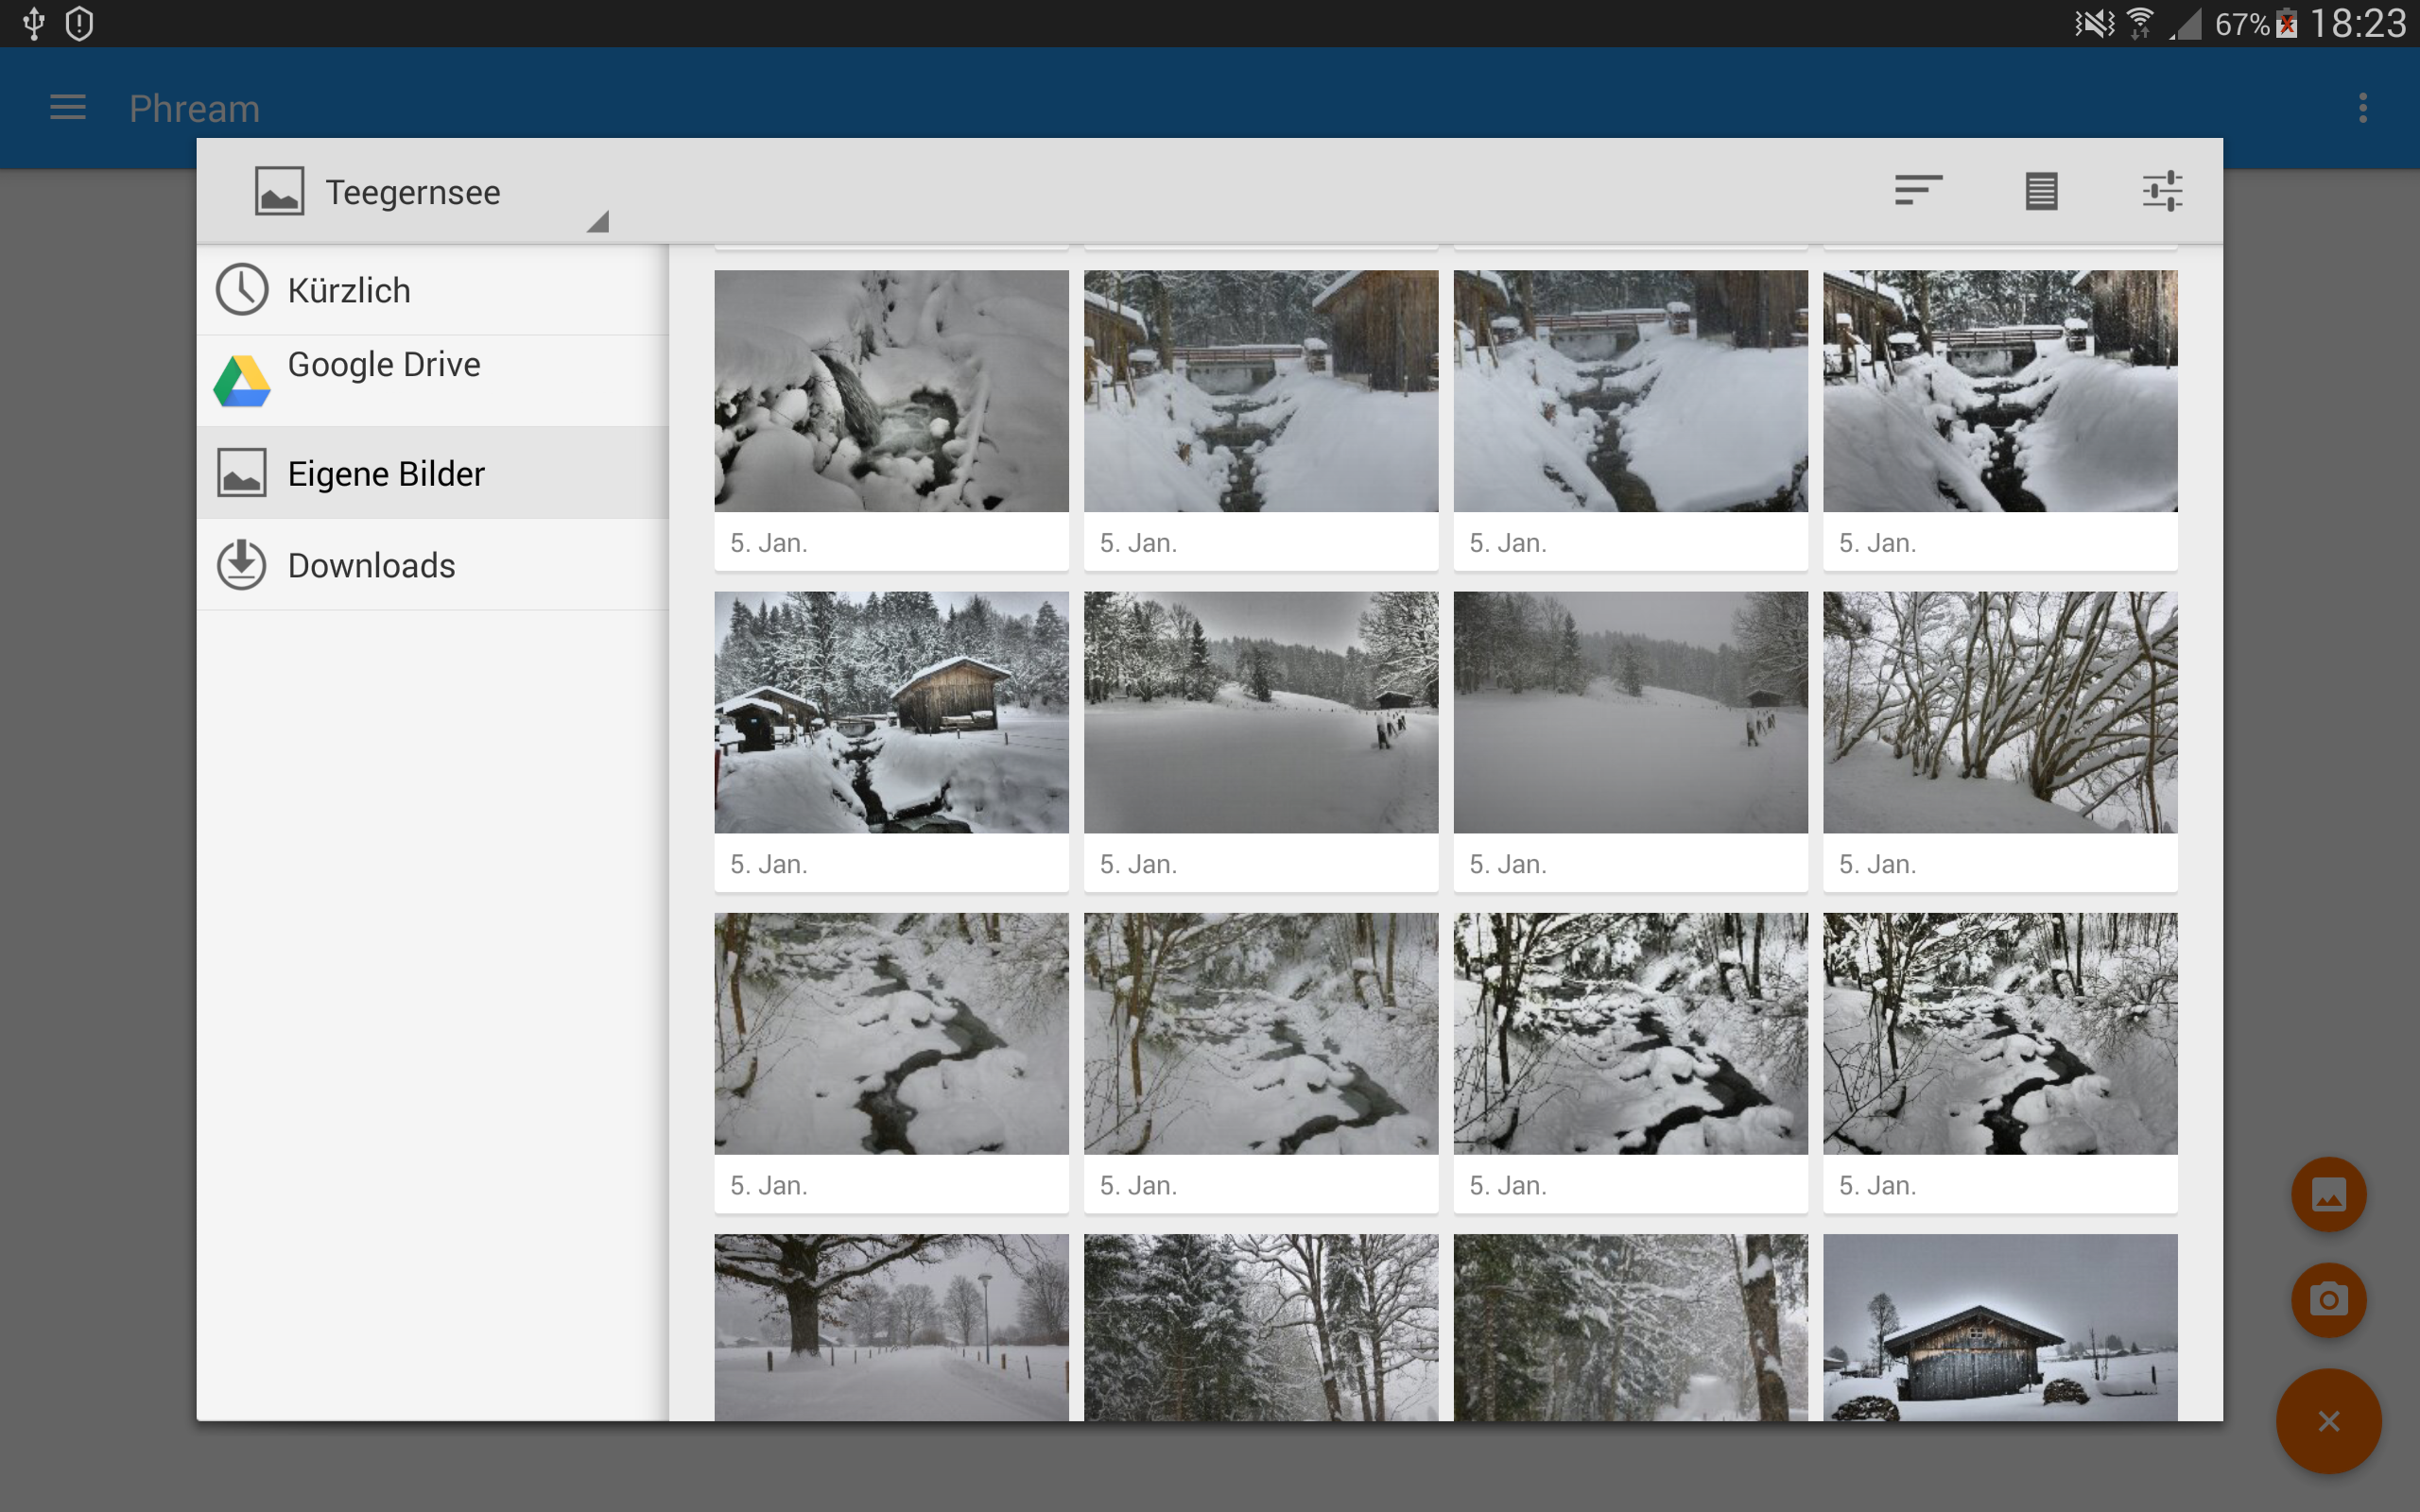
\includegraphics[scale=0.17]{images/screenshots/content_provider.png}
\caption{Content-Provider zum Auswählen eines Bildes}
\label{label:content_provider}
\end{figure}

\section{Verwendete Libraries}
Um verschiedene Benutzeroberflächenelemente auch auf früheren Android Versionen verfügbar zu machen, wurde die Support Library\footnote{\url{http://developer.android.com/tools/support-library/features.html}} von Google verwendet. Sie ermöglicht erst in späteren Android Versionen eingefügte Features auch unter älteren Anroid Geräten verfügbar zu machen. Weiterhin wurde zur Gestaltung des Floating Action Menu die AppCompat-Extension-Library\footnote{\url{https://github.com/TR4Android/AppCompat-Extension-Library}} verwendet, um einfach und schnell Floating Action Menu's zu gestalten. Beide Libraries ermöglichen, dass die App von API-Level 16 bis API-Level 22 verfügbar ist.

Aufgrund eines Bugs in der Standardexportfunktion von Android zum exportieren von Fotos in die Galerie, wurden exportierte Bilder immer am Ende der Galerie mit Datum 1.1.1970 angezeigt. Daher wurde die Klasse \enquote{CapturePhotoUtils}\footnote{\url{https://gist.github.com/samkirton/0242ba81d7ca00b475b9}} von samuelkirton zum Exportieren von Bildern verwendet.

	%!TEX root = ../documentation.tex

\chapter{Implementierung}

Viele implementieren Features beinhalten nur das einfache darstellen von Dialogen oder das Starten von Intents. Daher wird in diesem Abschnitt nur auf dem RecyclerView und dessen Verwendung eingegangen, da dieser eine tiefgründigere Dokumentation erfordert. 

Allgemein ist der RecyclerView eine Verbesserung des ListView's und dient der Darstellung von Informationen. Weiterhin bietet der RecyclerView eine bessere Performance gegenüber dem älteren ListView und ist freier gestaltbar. Zudem können einzelne Inhalte des RecyclerView's dynamisch ausgetauscht werden, ohne die komplette Ansicht neu zu laden. Um Inhalt darzustellen benötigt der RecyclerView  einen LayoutManager der den Inhalt verwaltet, einen RecyclerViewAdapter, indem der darzustellende Inhalt gespeichert wird und eine Activity / ein Fragment indem der Inhalt angezeigt wird. In diesem Projekt wurde als LayoutManager der Standardlayoutmanager \enquote{LinearLayoutManager} verwendet. Der RecyclerViewAdapter wurde selbst implementiert, um diesem auf die gegebenen Daten anzupassen. Der RecyclerViewAdapter beinhaltet die Klasse ViewHolder, von der für jedes angezeigte Objekt eine Instanz erzeugt wird. Im ViewHolder werden zum einem Referenzen auf das Layout des anzuzeigenden Inhalts gespeichert und zum anderen auf dem gespeicherten Layout Listener für Klick-Events definiert. In der Methode \enquote{onCreateViewHolder()} wird im RecyclerViewAdapter ein neuer ViewHolder angelegt und diesem das definierte CardLayout zugewiesen. Wenn das entsprechende Objekt auf dem Bildschirm des Nutzers aktiv ist (sprich angezeigt wird), ruft der LayoutManager die Methode \enquote{onBindViewHolder()} auf. In dieser Methode werden die anzuzeigenden Daten der Card geladen und beispielsweise auch das Vorschaubild durch einen \enquote{AsnycTask} erzeugt. Wird eine Card inaktiv (sprich wird nicht mehr angezeigt) wird das ViewHolder Objekt auf einen Stack gelegt. Sollte dieses Objekt wieder in den sichtbaren Bereich des Bildschirm kommen, versucht der RecyclerView, das alte Objekt wieder zu verwenden (zu recyclen). Dadurch steigt die Performance der App. 

Um dynamisch den Inhalt des RecylcerView austauschen bietet dieser verschiedene Methoden. Die einfachste Methode um den Inhalt zu tauschen, wenn man nicht weiß welche Inhalte geändert wurden, ist die Methode \enquote{mRecyclerView.swapAdapter(mAdapter, false)} mit einem neuen RecyclerViewAdapter aufzurufen. Dabei tauscht der RecyclerView nur neue / geänderte Elemente aus.

Um alle Benutzer Events auf dem RecyclerView Inhalt (den Cards) kümmert sich der der ViewHolder. Einfache Intent-Starts sind dadurch einfach zu realisieren. Komplexer wird dies, wenn die App wissen muss welche Card angetippt wurde, oder beispielsweise \enquote{long taps} registriert werden müssen, da der ViewHolder nicht von \enquote{View} erbt, sondern von \enquote{RecyclerView.ViewHolder}. Dieser stellt keine Implementierungen der Methoden \enquote{onCreateContextMenu} und \enquote{onContextItemSelected} bereit und zudem existiert zu den einzelnen Cards keine Code-Behind-Klasse. Daher wurde ein eigener RecyclerView implementiert, der den Standard RecyclerView um einen ContextMenuHolder erweitert und Informationen über das angeklickte Objekt speichert und somit eine Implementierung eines Kontextmenüs ermöglicht.


	% Anhang römsiche Ziffern für Verzeichnisse
	\clearpage
	\pagenumbering{roman}
	\setcounter{page}{3}
	
	%Tabellenverzeichnis falls benötigt
	%\cleardoublepage
	%\listoftables

	% Quellcodeverzeichnis falls benötigt
	%\cleardoublepage
	%\lstlistoflistings

	% Literaturverzeichnis
	\cleardoublepage
	\printbibliography[title=Literaturverzeichnis]
\end{document}